O Framework Decisioner organiza e generencia os componentes gerais
dos SADs de avaliação. Cada SAD tem particularidades que precisam
ser definidas e ajustadas para configurar suas funcionalidades. As
ontologias específicas do domínio e as DSL, explicadas nos capítulos
anteriores fornecem o meio de definição dessas particularidades. 

O SAD SustenAgro foi usado como a primeira instanciação do Framework
Decisioner. Ele é composto por uma ontologia de domínio, DSL e elementos
gráficos de design (ícones, imgens de fundo, etc.) que permitem instanciá-lo
no Decisioner. Sendo seu principal componente a ontologia do domínio
de avaliação da sustentabilidade da produção de cana-de-açucar na
região centro-sul do Brasil..

Nest capítulo, serão explicadas a arquitetura, a metodologia e os
componentes mais importantes do SAD SustenAgro. Serão feitas também
algumas considerações sobre o processo de definição do SAD.

\section{Arquitetura do SustenAgro}

O SAD SustenAgro serviu de base para modelar e desenvolver os componentes
que fazem parte do Decisioner. Por isso, o processo real de desenvolvimento
dele foi muito mais complicado que uma simples instanciação de um
framework. Ele envolveu diversas iterações para determinar o que deveria
ser implementado como parte do framework e como parte da aplicação.
Para simplificar o texto e facilitar o entendimento de como o framework
Decisioner é usado para instanciar um SAD, as diversas versões do
framework não serão discutidas.

Um SAD implementado usando o Decisioner tem os seguintes componentes:
\begin{enumerate}
\item Ontologia do domínio: ontologia que representa os conceitos do domínio.
No caso do SustenAgro, o domínio é a avaliação da sustentabilidade
do sistema produtivo de cana-de-açúcar, na região centro-sul. Essa
ontologia é a base para o SAD pois permite estabelecer os conceitos
fundamentais, que são utilizados pelo sistema. No caso do SustenAgro,
eles são: indicadores, componentes de indicadores, índices, dimensões
da sustentabilidade, recomendações e o método de avaliação.
\item DSL: programa descrevendo a configuração e comportamento do SAD. Ele
especifica as features do domínio a serem usadas, as fórmulas do modelo
e o aspecto e estrutura do relatório a ser gerado. No caso do SustenAgro,
as features são os indicadores, as formulas calculam os índices de
sustentabilidade e produtividade, e o relatório usa a Matriz e o Semáforo
de Sustentabilidade.
\selectlanguage{english}%
\item Web components\foreignlanguage{brazil}{: o SustenAgro usa duas widgets
específicas (além das oferecidas pelo Decisioner): a Matriz de Sustentabilidade
e o Semáforo de Sustentabilidade. Ambas são implementadas como Web
Components usando a biblioteca Polymer da Google.}
\selectlanguage{brazil}%
\item Imagens e layout: Um conjunto de imagens e arquivos de layout (css)
compõem o look-and-feel específico do SAD, incluindo seu logo.
\end{enumerate}

\section{Metodologia.\label{sec:Metodologia}}

O conhecimento do domínio abrangido no sistema SustenAgro está em
contínua evolução. Por isso, foi necessário usar uma metodologia que
suporte mudanças na estrutura e nos dados do sistema, durante cada
uma das fases do desenvolvimento. O desenvolvimento da ontologia de
domínio SustenAgro foi realizada de forma ágil e modular, por meio
de técnicas de prototipação rápida, abrangendo grupos de conceitos
relacionados entre si.

O desenvolvimento da ontologia depende essencialmente da comunicação
entre os especialistas de domínio e os modeladores. Dessa forma, foram
definidos meios de comunicação (reuniões presenciais e virtuais) e
de representação do conhecimento (modelos conceituais), que permitiram
explorar o domínio. 

Um dos meios, que permitiu uma melhor comunicação, foi o desenvolvimento
de um mapa conceitual, por meio da ferramenta Cmap Tools\footnote{http://cmap.ihmc.us/},
com a participação de um grupo de especialistas em modelagem de conhecimento.
Esse processo começou em uma reunião da equipe na Embrapa Informática
Agropecuária (situada situada na Universidade Estadual de Campinas,
UNICAMP). Nessa reunião, um especialista em desenvolvimento de ontologias
da Embrapa forneceu treinamento sobre a metodologia para definir ontologias,
desenvolvimento de mapas conceituais, com os principais conceitos,
e desenvolvimento de modelos em \foreignlanguage{english}{OWL,} para
tornar esse conehcimento computável.

Após realizada a modelagem, o especialista do domínio definiu perguntas
de interesse, com as quais os modeladores, eu e outro colega de mestrado,
definiram consultas que o sistema deveria responder segundo os resultados
esperados, conseguindo validar e ajustar o modelo até ter um protótipo
confiável.

Na Figura \ref{fig:Methodology} é apresentada a metodologia para
desenvolver a ontologia SustenAgro, a qual teve vários ciclos de desenvolvimento
nos quais foram integradas novas caraterísticas.

\begin{figure}[H]
\noindent \begin{centering}
\includegraphics[width=0.8\columnwidth]{\string"figures/Ontology Methodology\string".eps}
\par\end{centering}
\caption{Metodologia de definição da ontologia SustenAgro.\label{fig:Methodology}}
\end{figure}

Um aspecto importante das ontologias é que elas fornecem um formato
que adapta-se às mudanças do domínio e permite separar o conhecimento
dos outros componentes do sistema.

A metodologia, que direcionou o desenvolvimento do SAD SustenAgro,
foi \foreignlanguage{english}{a SCRUM} \citet{schwaber2002gile},
que permitu integrar práticas ágeis no desenvolvimento do sistema.
Nesse contexto, o termo ágil refere-se ao desenvolvimento em tempos
curtos e geração de protótipos facilmente adaptáveis às mudanças.
Cada uma das etapas da metodologia foi realizada várias vezes e, por
isso, foi necessário redesenhar os componentes. As metodologias ágeis
são cíclicas e os protótipos mudam em cada ciclo para cumprir os novos
requisitos.

\label{A-metodologia-de-UI}A metodologia de desenvolvimento dos \foreignlanguage{english}{Web
Components} e das \foreignlanguage{english}{Web UI} foi teve um enfoque
baseado em \foreignlanguage{english}{User Centered Design,} que permitiu
integrar esses dois elementos para avaliar se as interfaces satisfazem
os requisitos identificados. 

O processo de design das \foreignlanguage{english}{web UI} incluiu
as seguintes etapas de levantamento de requisitos:
\begin{enumerate}
\item Descrição de \foreignlanguage{english}{User Stories:} técnica de desenvolvimento
ágil que permite descrever características do software desde a perspectiva
do usuário. Ela fornece uma identificação dos usuários, das funcionalidades
e explica o porque uma dita funcionalidade é necessária. 
\item Descrição de \foreignlanguage{english}{Scenarios:} técnica de desenvolvimento
ágil que permite descrever detalhadamente as características das \foreignlanguage{english}{user
stories}.
\item Descrição de \foreignlanguage{english}{Storyboard\emph{s:}} descreve
cada uma das interações do usuário com o sistema em uma determinada
tarefa, visualizando a interação como uma história em quadrinhos.
\item Descrição de \foreignlanguage{english}{\emph{Mockups:}} design do
esboço da interface gráfica do sistema. Eles foram analisados pelos
especialistas da Embrapa, para avaliar se atendiam às funcionalidades
básicas descritas no levantamento dos requisitos.
\item Desenvolvimento de protótipo visual: A partir da validação dos \foreignlanguage{english}{Mockups,}
foi desenvolvido um protótipo da interface gráfica, com a finalidade
de que os especialistas do domínio avaliassem se as interfaces cumpriam
com os requisitos.
\end{enumerate}
Cada uma dessas etapas de desenvolvimento, foram realizadas sempre
em parceria com os especialistas do domínio. Isso foi importante para
realizar o levantamento correto de requisitos tanto das web UI como
das funcionalidades do SAD, identificadas a partir destas técnicas.
Todo esse processo foi necessário pois não existia uma definição especifica
do que os especialistas precisavam.

\section{Ontologia de domínio: SustenAgro\label{sec:Ontologia-do-dom=0000EDnio}}

A ontologia SustenAgro representa o conhecimento necessário para suportar
avaliação de sustentabilidade no sistema produtivo de cana-de-açúcar
na região centro-sul do Brasil. Ela representa conceitos por meio
de entidades, classes, relações semânticas e axiomas. Esses elementos
organizam e representam a realidade modelada. 

Para definir a ontologia SustenAgro, realizou-se uma pesquisa das
fontes de dados relacionadas com ontologias do domínio de avaliação
de sustentabilidade em sistemas produtivos de cana-de-açúcar. Concluiu-se
que não existem ontologias que suportassem esse domínio. Por isso,
propôs-se desenvolver uma ontologia que utilizasse conceitos sobre
avaliação de sustentabilidade e sistemas agrícolas. Essa ontologia
representa conceitos gerais de conceitos identificados na literatura
e conceitos particulares ao SustenAgro, identificados por \citet{oliveira:2013}.
Deve-se destacar que a ontologia SustenAgro abrange um domínio bem
específico: sustentabilidade de sistemas produtivos de cana-de-açucar
na região centro-sul do Brasil. Acreditamos que essa é uma característica
deste tipo de SAD. Modelamentos desse tipo tendem a ser específicos.
No caso do Sustenagro, ele abrange apenas um só sistema produtivo
em uma região específica.

A figura \ref{fig:ontology-conceptual-map} representa um mapa conceitual
com os principais conceitos modelados no SustenAgro e como eles estão
relacionados entre si. As etiquetas, em cada relação dos conceitos,
permitem identificar a relação entre os dois conceitos.

\begin{figure}[H]
\begin{centering}
\includegraphics[width=0.7\columnwidth]{\string"figures/SustenAgro conceptual map\string".eps}
\par\end{centering}
\caption{Mapa conceitual da ontologia SustenAgro.\label{fig:ontology-conceptual-map}}
\end{figure}

As ontologias da web semântica satisfazem o requisito de separar o
conhecimento do domínio da lógica da computação. Essa separação permite
que o desenvolvimento de cada parte seja feito de maneira independente
e suportando conceitos importantes como a inferência, que são de
grande importância no desenvolvimento de SAD.

Uma caraterística importante da ontologia SustenAgro é a recuperação
da informação com significado semântico, permitindo que o sistema
dê respostas às consultas complexas de interesse para os especialistas,
além da integração com conhecimento externo existente em formatos
da web semântica, como são os padrões \foreignlanguage{english}{RDF},
\foreignlanguage{english}{OWL} e vários sistemas de representação
do conhecimento como dicionários, \foreignlanguage{english}{thesaurus}
e redes semânticas, o que permite aumentar as possibilidades de integração
com diversas tecnologias e fornecer novas funcionalidades. 

Para conseguir que a ontologia SustenAgro fosse computável, foi necessário
defini-la na linguagem \foreignlanguage{english}{OW}L (fornecendo
uma representação compreensível por humanos e computadores). O editor
de ontologias Protégé\footnote{\url{http://protege.stanford.edu/}}
foi usado. O arquivo final foi exportado no formato \foreignlanguage{english}{RDF},
para melhor compatibilidade com sistemas \foreignlanguage{english}{triple-stores}
(seção \ref{subsec:Triplestore}) \citep{allemang2011semantic}. Triplestores
suportam a realização de consultas complexas para permitir a resposta
a perguntas de interesse aos usuários do sistema.

A ontologia do SustenAgro modela o conhecimento dos especialistas
baseando-se na ontologia do Decisioner (Figura \ref{fig:Modelagem-do-SAD}).
Ela inclui a ontologia Decisioner e define seus conceitoa a partir
de conceitos gerais da Decisioner. Isso é obrigatório, pois o código
do framework Decisioner entende os conceitos da ontologia SustenAgro
apenas porque eles também são conceitos válidos derivados da ontologia
Decisioner. Exemplos de conceitos/classes modelados são: \foreignlanguage{english}{\textit{Production
Unit}}\textit{, }\foreignlanguage{english}{\textit{Microregion, Indicator}}\textit{,}
\foreignlanguage{english}{\textit{Categorical}}. A partir dessas classes
foi possível desenvolver o modelo de dados em \foreignlanguage{english}{OWL}, 

As classes da ontologia SustenAgro são relacionados por meio de \foreignlanguage{english}{\textit{Object
Properties}} e \foreignlanguage{english}{\textit{Data Properties}}
que permitem vincular semanticamente as instâncias das classes. A
principal contribuição da ontologia do domínio é ser uma representação
semântica do conhecimento de domínio, tanto para os usuários como
para o sistema computacional, tornando-se um meio de comunicação entre
os especialistas de domínio e os programadores.

Nas próximas seçõe, serão apresentadas as principais classes modeladas
na ontologia do domínio de avaliação da sustentabilidade (SustenAgro).
\selectlanguage{english}%

\subsection*{Production Unit}

\selectlanguage{brazil}%
Representa as organizações que podem ser avaliadas pelo sistema SustenAgro.
Atualmente elas podem ser \textit{Fornecedores de cana-de-açúcar}
e / ou \textit{Usinas processadoras de cana-de-açúcar}. Cada processo
de avaliação requer dados que identifiquem as unidades produtivas
através de propriedades que as definam. Existem propriedades obrigatórias
como:
\selectlanguage{english}%
\begin{itemize}
\item hasAgriculturalProductionSystem\foreignlanguage{brazil}{: relaciona
o sistema de produção agrícola em avaliação.}
\selectlanguage{brazil}%
\item hasAvailabilityOfEvaluationResults: relaciona o tipo de disponibilização
dos resultados.
\item hasSugarcaneSource: relaciona a origem da cana.
\item harvestYear: define o ano da safra.
\item canavialLongevity: define a longevidade do canavial.
\end{itemize}
\selectlanguage{brazil}%
A Figura \ref{fig:Modelagem-unidade-produtiva} apresenta a modelagem
da classe \foreignlanguage{english}{Production Unit}, feita na ferramenta
Protégé.

\begin{figure}[H]
\noindent \begin{centering}
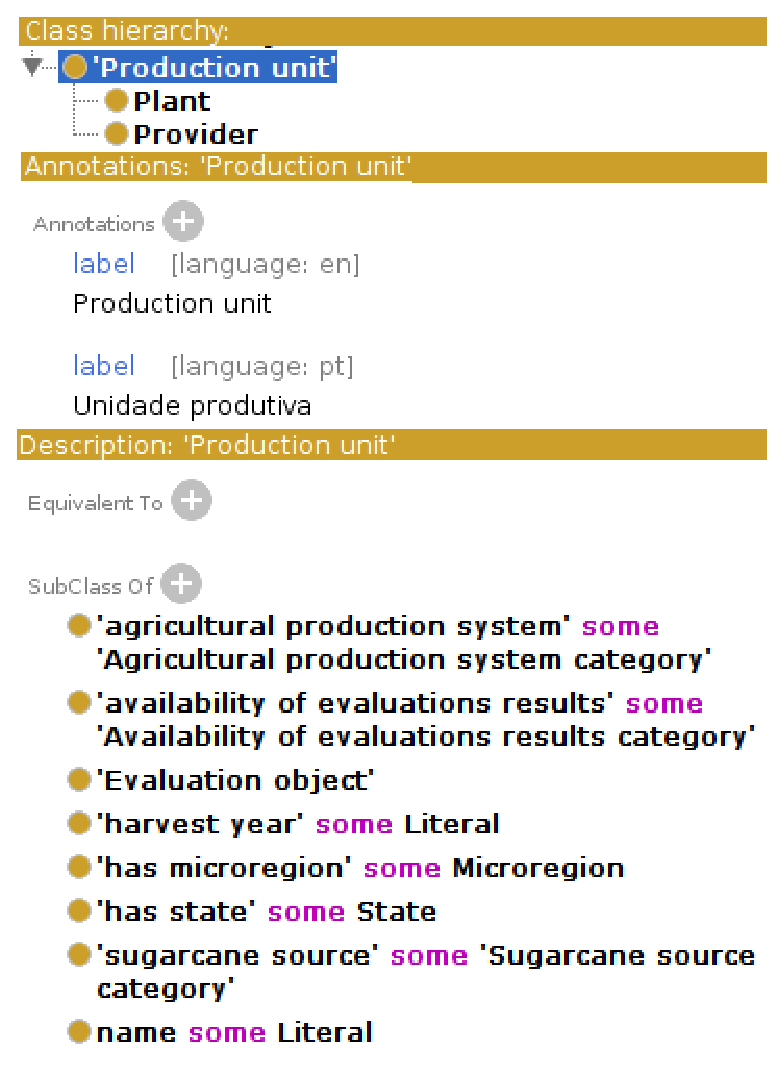
\includegraphics[width=0.6\columnwidth]{figures/ProductionUnit}
\par\end{centering}
\caption{Modelagem da classe de unidade produtiva (ProductionUnity). \label{fig:Modelagem-unidade-produtiva}}
\end{figure}

\selectlanguage{english}%

\subsection*{\textit{Microregion}\foreignlanguage{brazil}{\textit{ }}}

\selectlanguage{brazil}%
Representam os locais onde são localizadas as unidades produtivas.
É permitido definir a microrregião onde as fazendas e usinas do sistema
produtivo de cana-de-açúcar se localizam. Atualmente, a ontologia
tem os 7 estados pertencentes ao centro-sul do Brasil e as 243 microrregiões
dentro desses estados. Esses dados foram originalmente obtidos por
consulta SPARQL à DB-pedia e integrados à ontologia.

A Figura \ref{fig:Modelagem-de-Microrregi=0000E3o} mostra a modelagem
das localizações geográficas usadas no sistema SustenAgro, com algumas
instâncias de \foreignlanguage{english}{\textit{Microregion}}.

\begin{figure}[H]
\noindent \begin{centering}
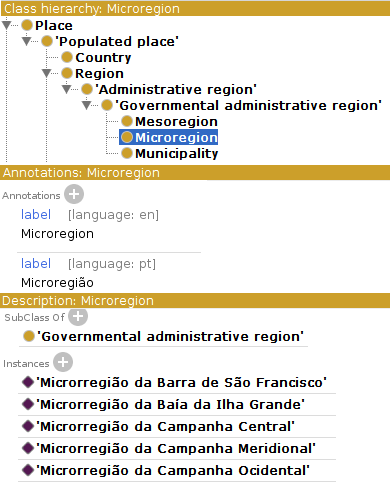
\includegraphics[width=0.6\columnwidth]{figures/Microregion}
\par\end{centering}
\caption{Modelagem de microrregiões.\label{fig:Modelagem-de-Microrregi=0000E3o}}
\end{figure}

\selectlanguage{english}%

\subsection*{\textit{Indicator}}

\selectlanguage{brazil}%
Os indicadores são o principal componente da ontologia. Eles foram
propostos por um grupo de especialistas de diversas áreas da produção
agrícola e sustentabilidade \citep{oliveira:2013}. 

Eles representam as características das unidades produtivas que serão
identificadas e quantificadas em cada processo de avaliação. Eles
tem uma propriedade \foreignlanguage{english}{\textit{Value}}\textit{
}que quantifica a sustentabilidade do indicador.

Também permite a integração de conceitos, inclusive quando pertencem
a domínios sem relação aparente. Um exemplo disso é a inter-relação
do conhecimento de sustentabilidade com conhecimento de interfaces
gráficas de usuário, que suporta a geração de SAD para avaliação da
sustentabilidade. O conhecimento foi dividido em duas ontologias,
avaliação de sustentabilidade e outra dos componentes gerais de um
SAD.

A Figura \ref{fig:Modelagem-de-Indicador} apresenta a hierarquia
dos indicadores, que está subdividida em \foreignlanguage{english}{Efficiency
Indicator} e \foreignlanguage{english}{Sustainability Indicator}.
Os \foreignlanguage{english}{Indicators} têm a propriedade \foreignlanguage{english}{\textit{has
value}}\textit{ }que estabelece um valor\textit{ .} Existe outra
propriedade, \foreignlanguage{english}{has weight,} que é opcional
e estabelece um peso para o indicador\foreignlanguage{english}{\textit{.}}

A Figura \ref{fig:Modelagem-de-Indicador} mostra o indicador intitulado
\foreignlanguage{english}{\textit{Adequacy of boilers}}. Na propriedade
\foreignlanguage{english}{\textit{has value}} ele tem uma restrição
que limita os valores dessa propriedade a valores de uma lista de
valores categóricos. A propriedade \foreignlanguage{english}{\textit{has
weight}} também tem uma restrição que limita seus valores a instâncias
da classe \foreignlanguage{english}{\textit{Sugarcane process Optimization}}.

\begin{figure}[H]
\noindent \begin{centering}
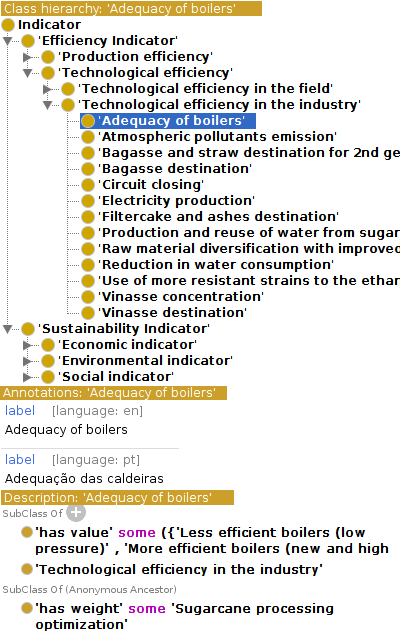
\includegraphics[width=0.6\columnwidth]{figures/Indicador}
\par\end{centering}
\caption{Modelagem de indicador \label{fig:Modelagem-de-Indicador}}
\end{figure}

Segundo a descrição do método de avaliação (Capítulo \ref{chap:Sustainability_Assessment}),
os indicadores de sustentabilidade são classificados em três dimensões
de sustentabilidade: dimensão ambiental, dimensão social e dimensão
econômica. Tendo as três uma participação equitativa no método de
avaliação \citep{kraines2011system}. 

A Figura \ref{fig:environment} representa a dimensão de indicadores
ambientais, de onde foram definidos os seguintes conceitos:

\begin{figure}[H]
\begin{centering}
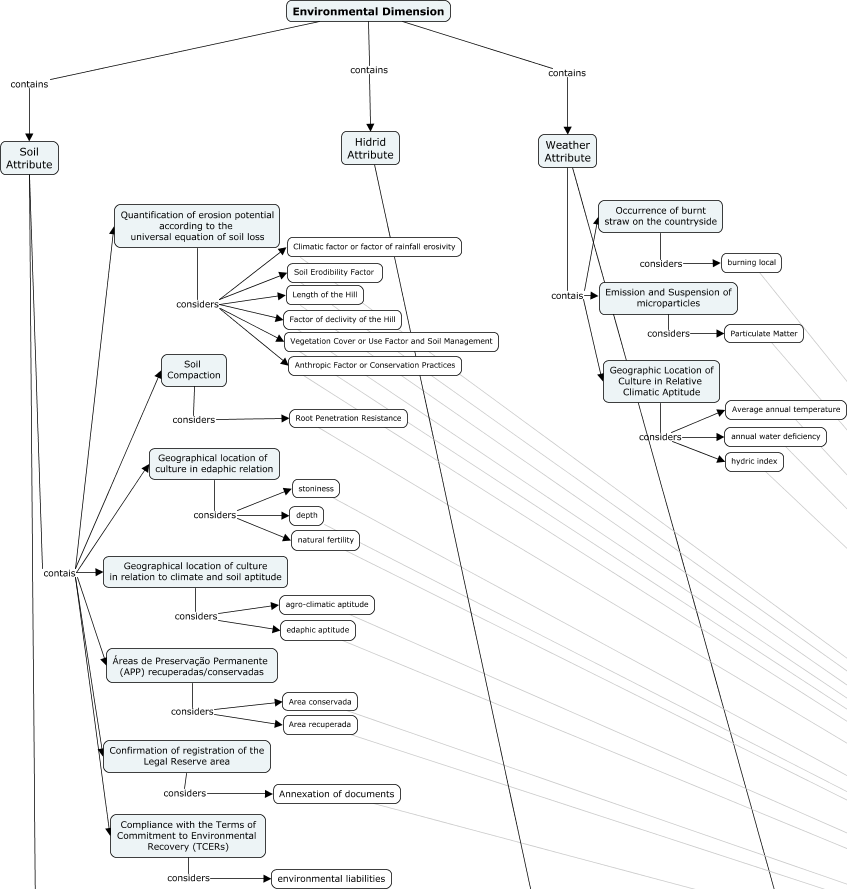
\includegraphics[width=1\textwidth]{figures/ambiental}
\par\end{centering}
\caption{Mapa conceitual - Dimensão Ambiental.\label{fig:environment}}
\end{figure}

\begin{itemize}
\item Atributo solo (\foreignlanguage{english}{Soil Attribute}): indicadores
que avaliam os aspectos referentes às características do solo.
\item Atributo hídrico (\foreignlanguage{english}{Hydric Attribute}): indicadores
que avaliam os aspectos referentes à disponibilidade e qualidade das
fontes hídricas.
\item Atributo clima (\foreignlanguage{english}{Weather Attribute}): indicadores
que avaliam os aspectos climáticos.
\end{itemize}
Nessa dimensão (ambiental), não foi possível identificar indicadores
de tipo hídrico. Não existe consenso entre os especialistas consultados
sobre quais são os aspectos mais relevantes deles para a avaliação
da sustentabilidade, porém, é um aspecto fundamental para trabalhar
nas futuras etapas de pesquisa.

A Figura \ref{fig:social} mostra a dimensão social, onde são definidos
os seguintes conceitos:

\begin{figure}[H]
\centering{}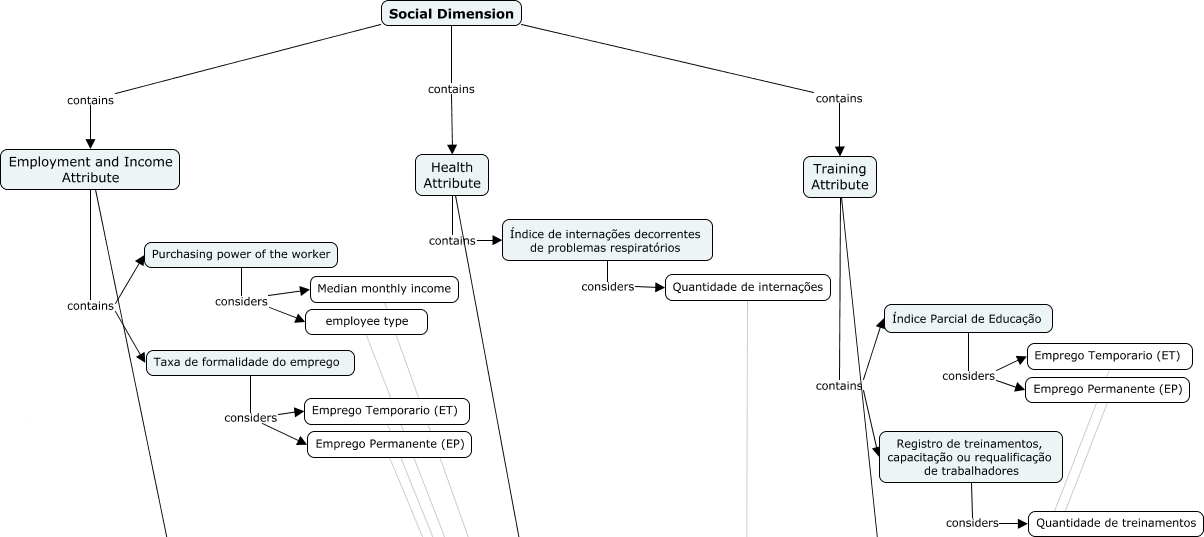
\includegraphics[width=1\textwidth]{figures/social}\caption{Mapa conceitual - Dimensão Social.\label{fig:social}}
\end{figure}

\begin{itemize}
\item Atributo emprego e renda (\foreignlanguage{english}{Employment and
Income Attribute}): indicadores que avaliam os aspectos referentes
à mão de obra.
\item Atributo saúde (\foreignlanguage{english}{Health Attribute}): indicadores
que avaliam os aspectos de segurança dos trabalhadores.
\item Atributo treinamento (\foreignlanguage{english}{Training Attribute}):
indicadores que avaliam os aspectos da capacitação dos trabalhadores.
\end{itemize}
Nessa dimensão (Social), é importante reconhecer que as unidades produtivas,
sejam do tipo fazendas ou usinas, têm vínculos com pessoas tanto internamente
como externamente. Por isso, é importante refinar os indicadores para
incluir a população externa à unidade produtiva que é afetada pelas
práticas produtivas.

A Agência Paulista de Tecnologia dos Agronegócios (APTA\nomenclature{APTA}{Agência Paulista de Tecnologia dos Agronegócios})
forneceu dados econômicos das principais usinas do estado de São Paulo,
que permitiram definir a dimensão econômica das unidades produtivas
na ontologia de domínio.

As Figuras \ref{fig:Economic-1} e \ref{fig:Economic-2} apresentam
a dimensão econômica, onde foram definidos os seguintes conceitos:

\begin{figure}[H]
\begin{centering}
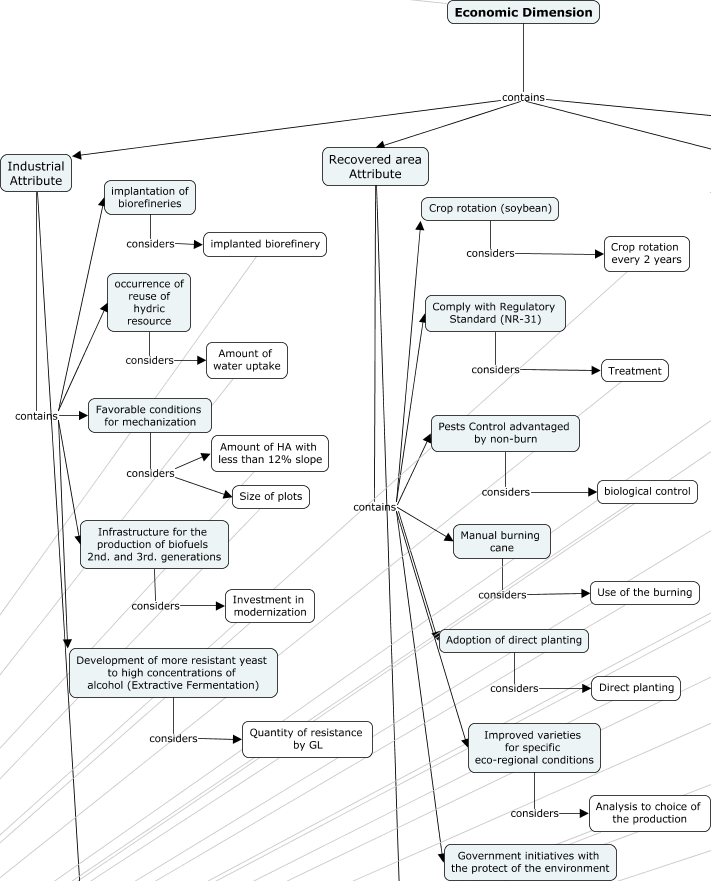
\includegraphics[width=1\textwidth]{figures/economica_1}
\par\end{centering}
\caption{Mapa conceitual - Dimensão Econômica (primeira parte).\label{fig:Economic-1}}
\end{figure}

\begin{figure}[H]
\begin{centering}
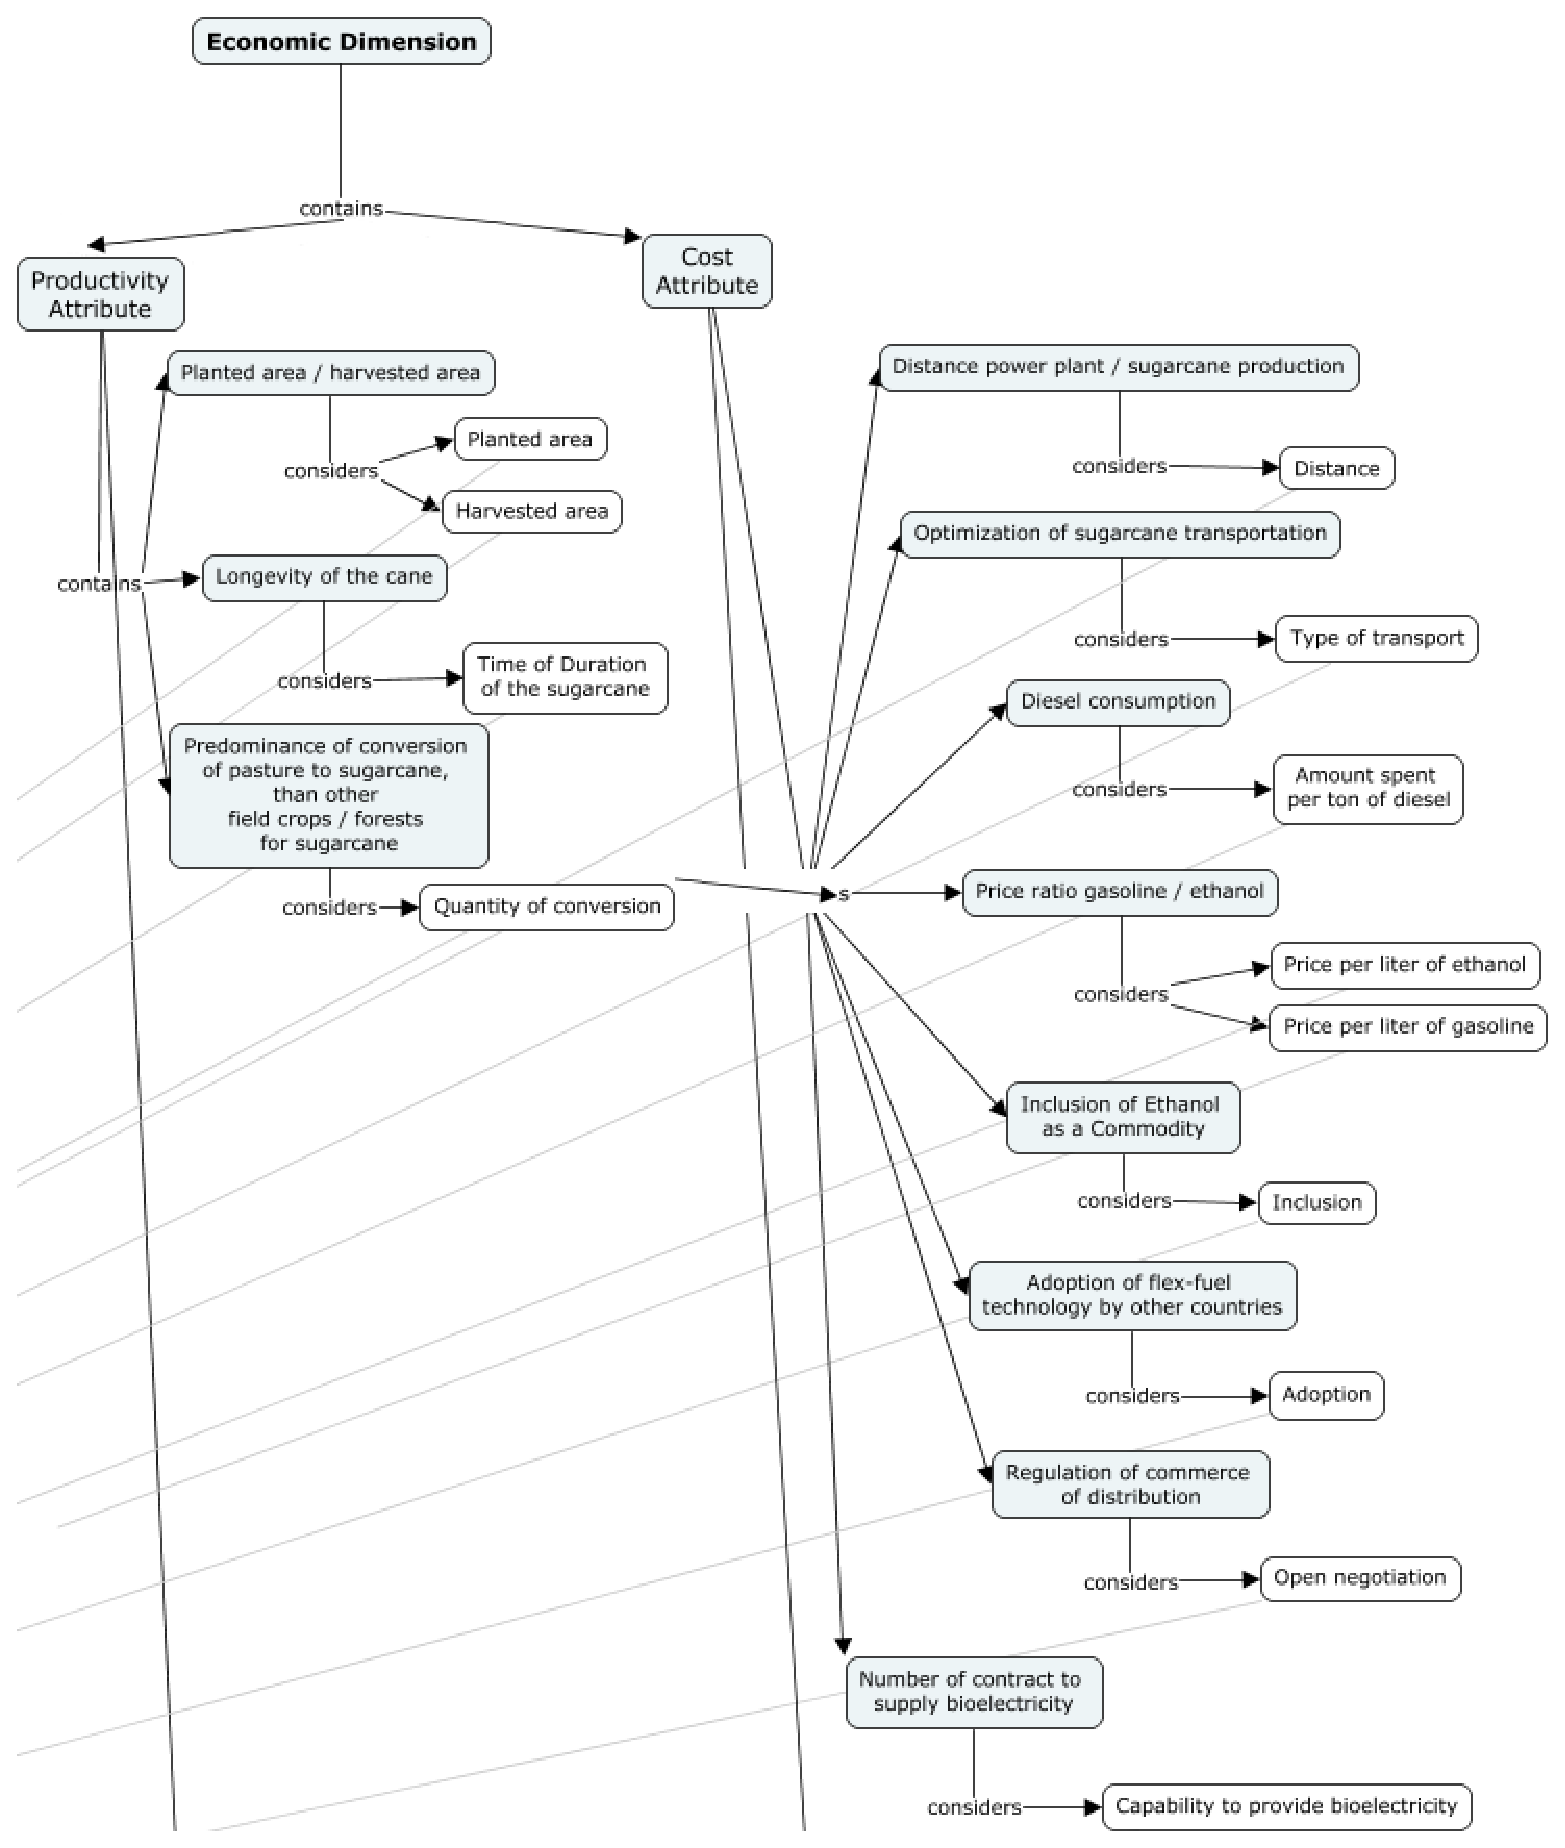
\includegraphics[width=1\textwidth]{figures/economica_2}
\par\end{centering}
\caption{Mapa conceitual - Dimensão Econômica (segunda parte).\label{fig:Economic-2}}
\end{figure}

\begin{itemize}
\item Atributo industrial (Industrial Atribute): indicadores que avaliam
os aspectos industriais. 
\item Atributo área recuperada (Recovered Area Atribute): indicadores que
avaliam os aspectos da área produtiva e das técnicas produtivas.
\item Atributo produtividade (Porductivity Atribute): indicadores que avaliam
os aspectos dos produtos e dos processos produtivos.
\item Atributo custo (Cost Atribute): indicadores que avaliam os aspectos
dos custos da produção. 
\end{itemize}
Cada uma das três dimensões deve ser avaliada equitativamente para
gerar um resultado coerente com a teoria da sustentabilidade agrícola\citep{tilman2002agricultural}.
A Figura \ref{fig:Method} mostra os conceitos envolvidos na avaliação
da sustentabilidade, fazendo uma integração entre os indicadores e
o método de avaliação. Cada um dos indicadores tem componentes de
indicadores que serão processados pelo método de avaliação, permitindo
quantificar a sustentabilidade.

\begin{figure}[H]
\begin{centering}
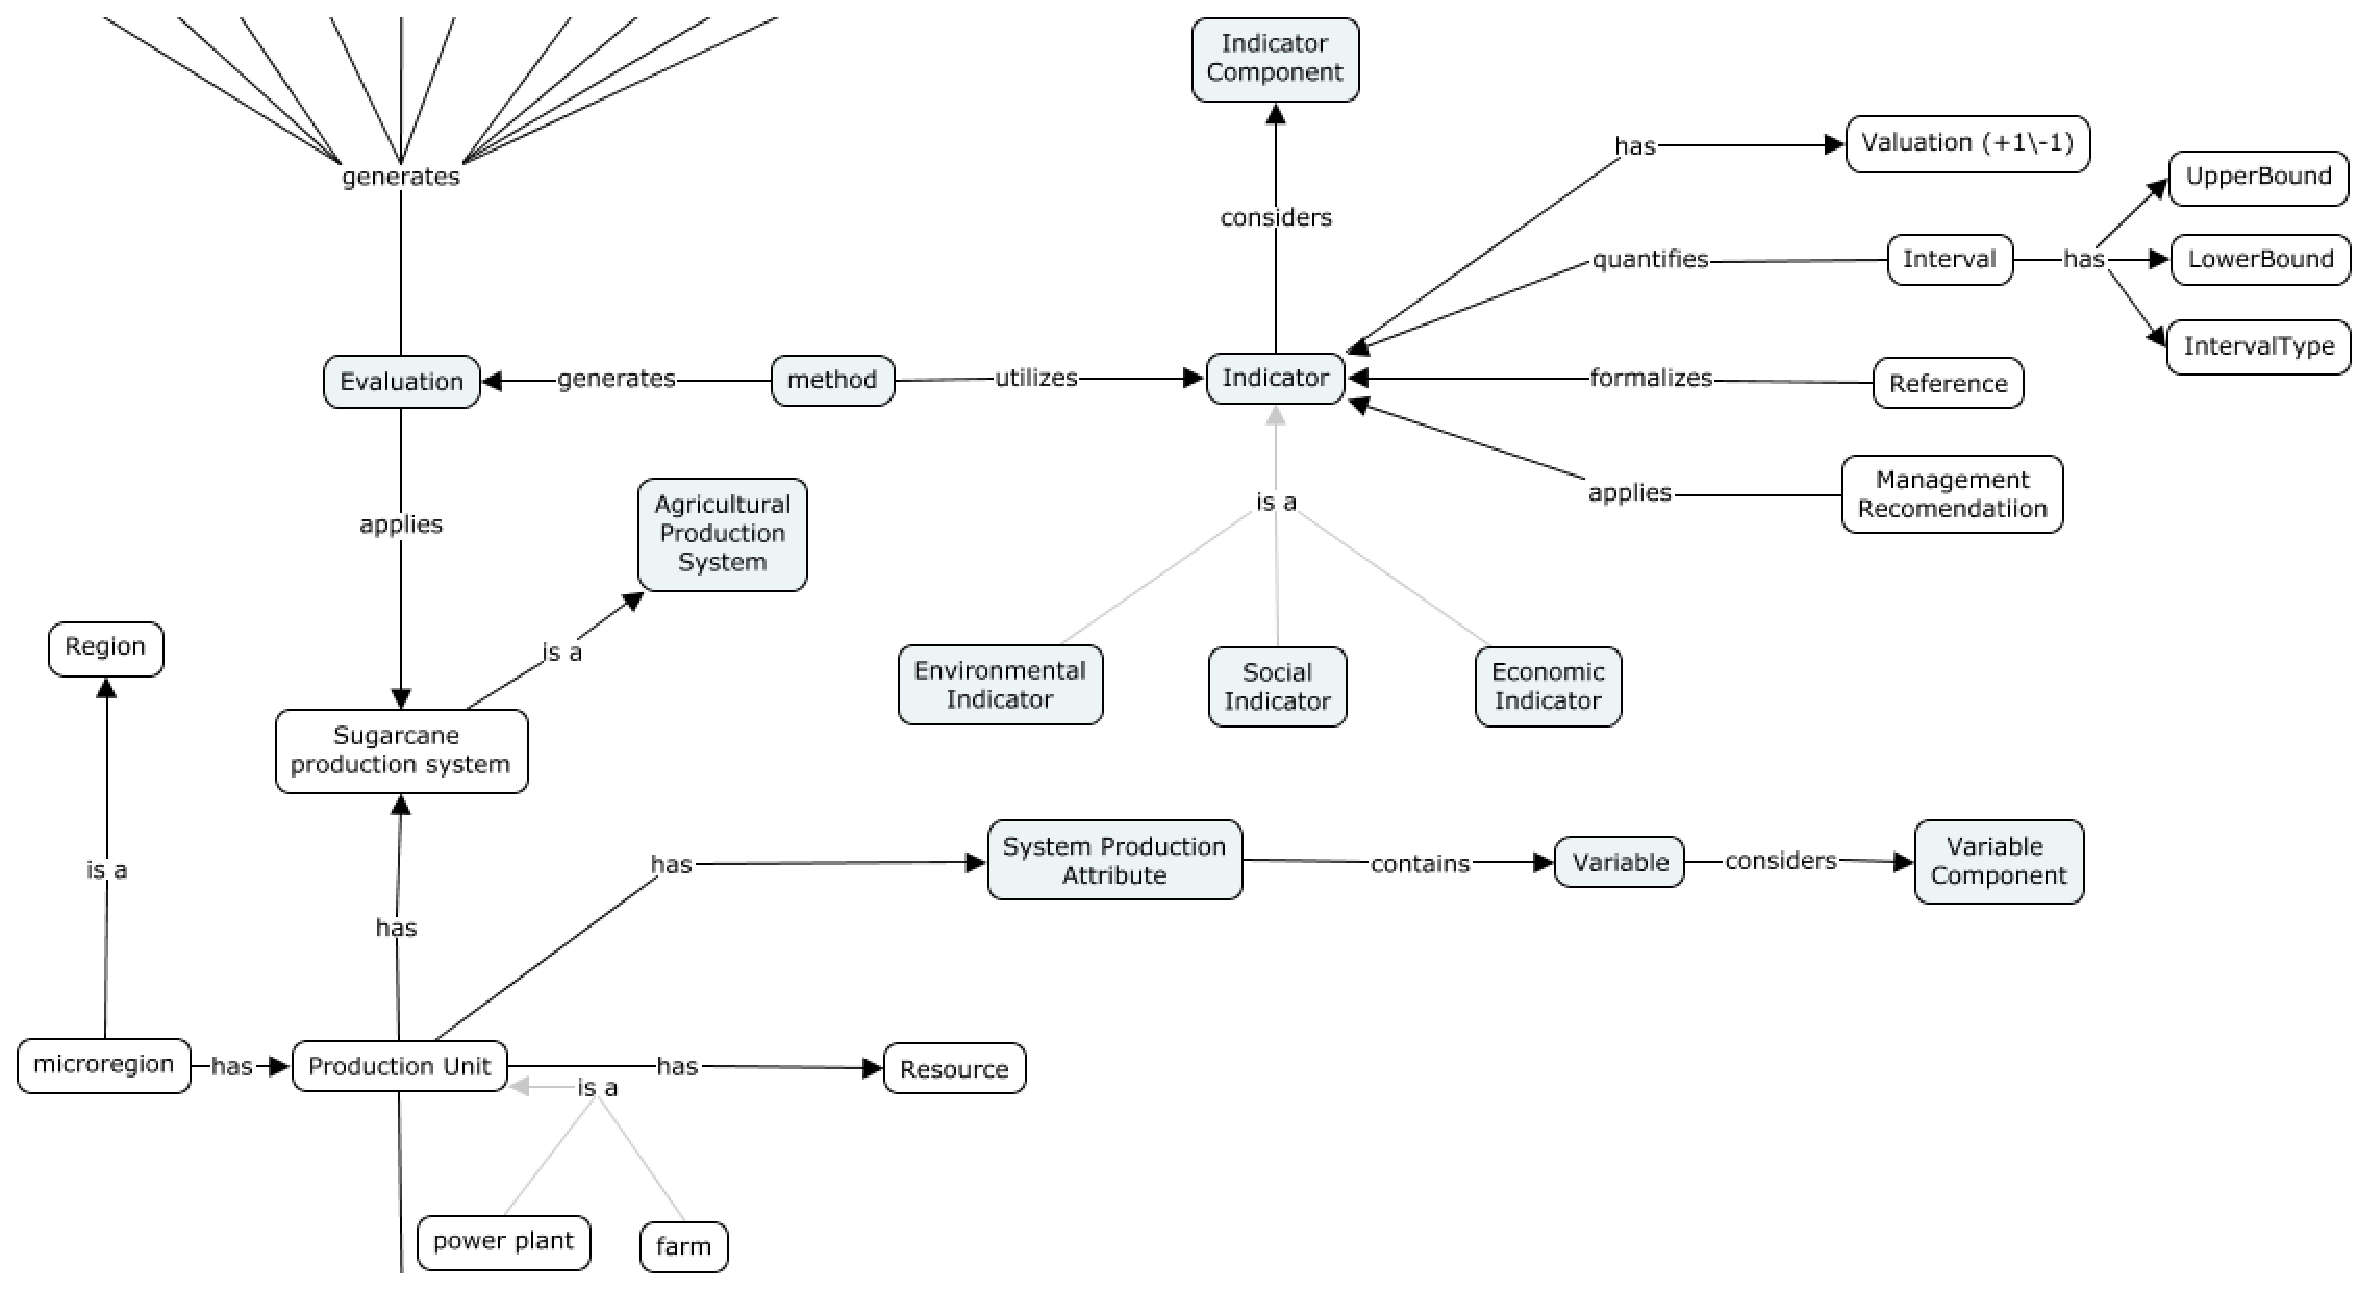
\includegraphics[width=1\textwidth]{figures/metodo}
\par\end{centering}
\caption{Mapa conceitual - Método de Avaliação.\label{fig:Method}}
\end{figure}

As dimensões da sustentabilidade permitiram organizar os indicadores,
levando essa organização desde os modelos de mapas conceituais, às
ontologias, método de avaliação e, finalmente, até a representação
dos resultados nas web UI dos SADs.
\selectlanguage{english}%

\subsection*{Categorical}

\selectlanguage{brazil}%
O conceito \foreignlanguage{english}{Categorical} representa os possíveis
\foreignlanguage{english}{Value} que um \foreignlanguage{english}{\textit{Indicator}}
ou \foreignlanguage{english}{\textit{Variable}} pode ter na forma
de categorias (por exemplo, Existe e Não Existe). Um Value também
pode ser Real ou Inteiro. Na verdade, a classe Categorical é definida
na ontologia Decisioner, mas a SustenAgro cria diversas classes filhas
para definir uma série de valores categóricos.

Cada subclasse de Categorical é composta por um conjunto finito de
elementos ou valores. Cada valor é modelado como indivíduo da classe,
permitindo assim, restringir as opções de instanciação de cada indicador.

Na Figura \ref{fig:Modelagem-de-Value}, é apresentada a classe \foreignlanguage{english}{\textit{Value}}
e suas subclasses, tanto \foreignlanguage{english}{\textit{Categorical}}
para conjunto finito de valores e \foreignlanguage{english}{\textit{Real}}
para valores numéricos. Um exemplo de classe categórica seria a \foreignlanguage{english}{\textit{Yes/No}}
que representa os valores de sim e não e é composta pela lista de
indivíduos Yes e No.

Cada individuo da classe \foreignlanguage{english}{\textit{Value}}
tem a propriedade \foreignlanguage{english}{\textit{as number}}\textit{
}que relaciona a ele um valor numérico. Esse valor define um critério
de comparação entre os indivíduos da mesma classe. Ele é usado nas
fórmulas do método de avaliação.

\begin{figure}[H]
\begin{centering}
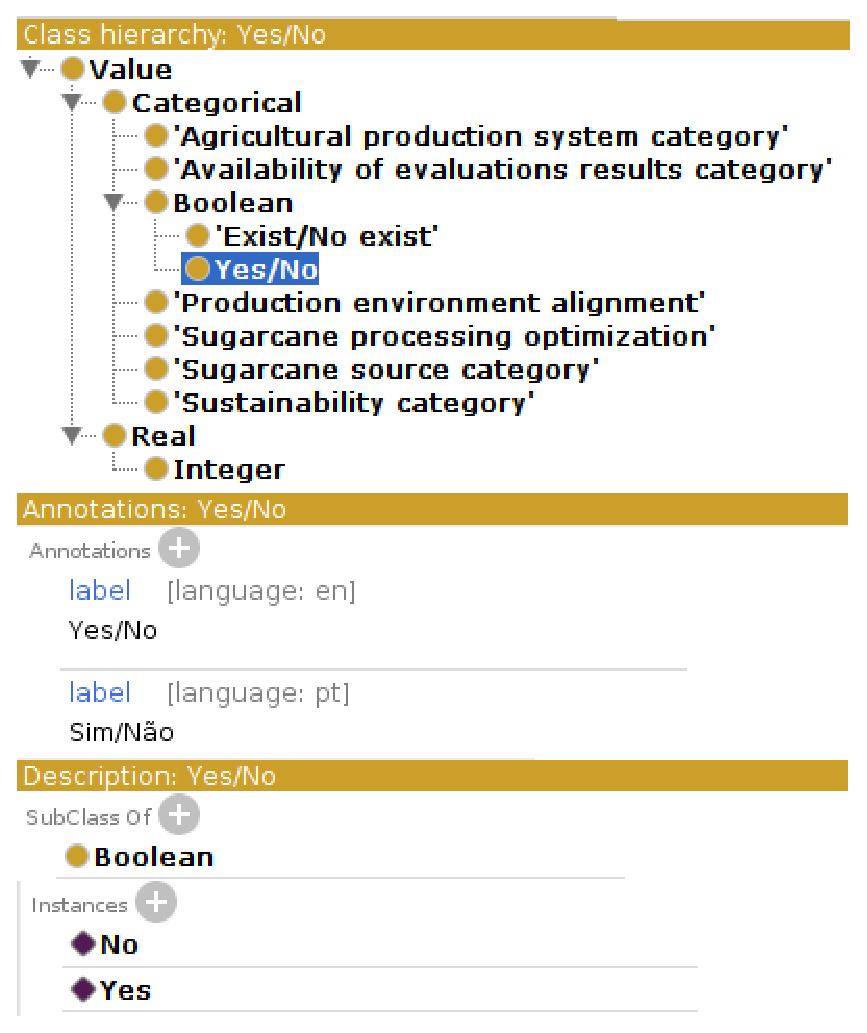
\includegraphics[scale=0.6]{figures/Value}
\par\end{centering}
\caption{Modelagem de \foreignlanguage{english}{Value}\label{fig:Modelagem-de-Value}}
\end{figure}

\selectlanguage{english}%

\section{SustenAgro Web UI\label{sec:Web-UI}}

\selectlanguage{brazil}%
O design das interfaces gráficas e desenvolvimento dos web componentes
foram realizados por meio da várias técnicas de levantamento de requerimentos
para especificar as funcionalidades que os especialistas precisavam
do sistema SustenAgro. Foram usadas as seguintes técnicas: \foreignlanguage{english}{User
Stories}, \foreignlanguage{english}{Scenarios}, \foreignlanguage{english}{Storyboard},
\foreignlanguage{english}{Mockups} e protótipo de interface gráfica.

Na fase inicial, foram definidos os perfis de usuários do SAD SustenAgro,
inicialmente definiram-se os perfis descritos a seguir: 
\begin{itemize}
\item Administrador: usuário com permissões para editar Ontologias, DSL
e web UI. Ele é o responsável pela administração do SAD e tem todas
as permissões do sistema.
\item Especialista de domínio: especialista em sustentabilidade ou afins,
com permissões para recuperar e gerenciar informações das avaliações,
gerar reportes e mudar os conceitos relacionados com os indicadores
e método de avaliação.
\item Usuário final: usuário padrão do sistema que tem permissões para realizar
avaliações de sustentabilidade em cana-de-açúcar e de gerenciar os
dados cadastrados por ele. 
\end{itemize}
No SAD SustenAgro v1.0, foi removido o perfil especialista, ficando
apenas os perfis administrador e usuário final. As funções desse perfil
foram incluídas no perfil administrador.

As técnicas realizadas para desenvolver as web UI, são descritas a
seguir.
\selectlanguage{english}%

\subsection*{User Stories}

\selectlanguage{brazil}%
Histórias de usuário são uma técnica para descrever, de uma forma
curta e simples, as características do sistema a partir da perspectiva
do usuário ou cliente do sistema, gerando uma definição de alto nível
de um requisito. O padrão é: como um “tipo de usuário”, eu quero atingir
“algum objetivo” para “alguma finalidade”.

Na aplicação dessa técnica foram obtidas as seguintes histórias:
\begin{enumerate}
\item O usuário poderá identificar e cadastrar a localização geográfica
e a área da sua lavoura (definir região geográfica do IBGE, latitude
e longitude - a partir do \foreignlanguage{english}{Google Maps}). 
\item O usuário poderá identificar e cadastrar a microrregião a que pertence
a sua lavoura. O sistema fará uma sugestão de cadastro a partir dos
dados da localização geográfica.
\item O usuário deverá preencher o estado de cada indicador específico nas
dimensões ambiental, econômica e social, devendo adaptar-se às condições
das regiões e microrregiões do Brasil.
\item O usuário poderá obter o resultado dos índices, segundo a informação
preenchida e a fórmula de agregação dos indicadores.
\item O usuário poderá armazenar a informação dos indicadores para futuras
consultas.
\item O usuário poderá acrescentar indicadores que considere importantes
para a análise. Deve-se estabelecer regras para essa funcionalidade
de tal modo que os novos indicadores (criados pelos usuários) sejam
recuperáveis de um modo separado dos indicadores cadastrados no sistema. 
\item O sistema deve fornecer um cronograma de avaliação, sendo recomendado
realizar a avaliação depois de cada safra.
\end{enumerate}
O usuário pode empregar a metodologia de avaliação caso a caso: possibilitando
que o usuário selecione quais indicadores vai utilizar, podendo recomendar
limiares mais adequados para a realidade dele e também inserir novos
indicadores/limiares. Finalmente, o usuário deverá ser informado da
importância dos processos de avaliação, exemplo: 
\begin{itemize}
\item “A crescente demanda de países desenvolvidos por produtos com garantia
de origem tem induzido aumento das certificações nas usinas no Brasil
(ALVES et al., 2008).” 
\item A certificação tem sido uma importante forma de diferenciação de commodities
agrícolas, facilitando seu acesso aos mercados protegidos dos países
desenvolvidos. 
\item A caracterização climática, aliada aos detalhes de fertilidade e manejo
do solo (quantificação edafoclimática), são essenciais para a determinação
das regiões aptas ao cultivo de culturas de interesse comercial (CIIAGRO,
2009). 
\end{itemize}
Depois do ingresso da informação sobre os indicadores, o usuário receberá
recomendações classificadas sobre práticas de sustentabilidade recomendadas
com sua argumentação, exemplo: 
\begin{itemize}
\item (Ambiental) “O sistema de plantio direto da cana-de-açúcar sobre leguminosas
proporciona maiores teores foliares de N e K na cana do que o plantio
convencional (JÚNIOR; COELHO, 2008)”.
\item (Ambiental) Segundo Leme (2005), haveria redução de 36\% na emissão
de gases do efeito estufa (GEE) se a palha fosse queimada nas caldeiras
das usinas e destilarias, ao invés de ser queimada no campo.
\item (Ambiental) A queima da cana aumenta a erosão do solo e a poluição
do ar e reduz a qualidade da matéria-prima (LINS; SAAVEDR, 2007). 
\item (Ambiental) Quando a cana não é queimada, proliferam, nos canaviais,
roedores silvestres originários de fragmentos florestais. Esses roedores
podem transmitir o Hantavírus através da urina e contaminar cortadores
de cana, causando uma síndrome respiratória e cardíaca, a pneumocitose,
podendo levar à morte. 
\item (Ambiental) Quando não há queima da cana é comum, também, o aumento
do ataque de cigarrinhas, com perdas significativas de produção (ANDRADE;
DINIZ, 2007). 
\item (Econômico) A utilização das colheitadeiras reverte-se em aumento
da produtividade e da qualidade da matéria-prima, bem como em diminuição
dos custos da produção agrícola, que representam entre 50\% e 60\%
em relação ao custo total (SCOPINHO, 1995).
\item (Econômico e Social) A utilização das colheitadeiras em cooperativa
possibilita a soma das áreas de produtores próximos possibilitando
a mecanização em propriedades com restrição para mecanização.
\item (Econômico) Restrições físicas da propriedade (menos de 500 ha de
área com declividade inferior a 12\% e talhões menores que 800 metros)
dificultam a mecanização. 
\end{itemize}
\selectlanguage{english}%

\subsection*{Scenarios}

\selectlanguage{brazil}%
É uma técnica que permite a descrição das funcionalidades do sistema
desde a perspectiva do usuário ou cliente, realizando uma descrição
detalhada de cada um dos passos dos usuários no sistema para completar
uma tarefa. A seguir serão apresentadas as 8 histórias de usuários
do SAD SustenAgro com os cenários associados:

\textbf{História de usuário \#1:} “O usuário poderá identificar e
cadastrar a localização geográfica e a área da sua lavoura (definir
região geográfica do IBGE, latitude e longitude - a partir do \foreignlanguage{english}{Google
Maps}).”
\begin{enumerate}
\item O usuário ingressa na conta dele, através do sistema web SustenAgro
em \url{http://sustenagro.embrapa.br}, e o sistema apresenta a tela
“\foreignlanguage{english}{Home}” 
\item O usuário seleciona a aba “unidades produtivas” e dá um \foreignlanguage{english}{click}
em ``cadastrar unidade produtiva'', o sistema apresenta a tela de
cadastro de unidades produtivas, onde tem um mapa do \foreignlanguage{english}{Google
Maps} 
\item O usuário seleciona no mapa um ponto que identificará a localização
da unidade produtiva, se ele quiser, também é possível marcar a área
da lavoura para que o sistema possa ter dados mais específicos para
o processo de avaliação de sustentabilidade. Uma vez terminado, o
usuário dá um \foreignlanguage{english}{click} no botão “próximo”
e o sistema cadastra a informação preenchida. 
\end{enumerate}
\textbf{História de usuário \#2}: “O usuário poderá identificar e
cadastrar a microrregião a que pertence a unidade produtiva dele,
por meio de uma sugestão que o sistema faz com os dados da localização
geográfica.”
\begin{enumerate}
\item O usuário poderá fazer a “Historia de usuário \#1” ou entrar no sistema
e continuar com o cadastro da unidade produtiva de onde ele tenha
parado. O sistema apresentará uma tela com sugestões de microrregiões. 
\item O usuário poderá escolher a microrregião, onde esteja localizada a
unidade produtiva, e salvá-la no sistema por meio do botão ``próximo''. 
\end{enumerate}
\textbf{História de usuário \#3:} “O usuário deverá preencher o estado
de cada indicador específico nas dimensões ambiental, econômica e
social. Esses indicadores devem adaptar-se às condições das regiões
e microrregiões do Brasil, da mesma forma as faixas de limiares de
sustentabilidade foram definidas.''
\begin{enumerate}
\item O usuário poderá fazer a “História de usuário \#2” ou entrar no sistema
e continuar com o cadastro dos indicadores de onde ele tenha parado.
O sistema apresentará uma tela com três abas que contém os controles
que permitirão fazer o cadastro dos indicadores nas dimensões ambiental,
econômica e social. 
\item O usuário dá um \foreignlanguage{english}{click} na primeira aba e
começa a preencher os dados dos indicadores ambientais, principalmente
os limiares que identificam o estado do indicador. A interface também
permite eliminar ou acrescentar indicadores específicos, por parte
dos usuários (funcionalidade que é explicada na “Hstória de usuário
\#4”). 
\item O usuário preenche os dados das outras duas dimensões e o sistema
salva as mudanças.
\end{enumerate}
\textbf{História de usuário \#4:} “Permitir o emprego da metodologia
para avaliação caso a caso: possibilitar que o usuário selecione quais
indicadores vai utilizar. Dentro dos indicadores, ele pode recomendar
limiares mais adequados para a sua realidade, também pode inserir
novos indicadores\slash{}limiares.”
\begin{enumerate}
\item O usuário poderá fazer a “Historia de usuário \#3” ou entrar no sistema
e continuar na tela de cadastro de indicadores e, quando aconteçer
que o usuário precise de um indicador que não seja oferecido pelo
sistema, o usuário poderá acrescentá-lo por meio do botão “acrescentar
indicador” 
\item O usuário dá um \foreignlanguage{english}{click} no botão “acrescentar
indicador” e lhe é apresentada uma interface de entrada, onde ele
deverá cadastrar o título, a descrição, os limiares, a medida do manejo
e a justificativa desse indicador. Em seguida preencher o estado do
indicador. O sistema salva esses dados nessa dimensão. 
\item O usuário também poderá eliminar alguns indicadores segundo seu critério.
\end{enumerate}
\textbf{História de usuário \#5:} \textquotedbl{}O usuário poderá
obter o resultado dos índices segundo a informação preenchida e a
formula de agregação dos indicadores.\textquotedbl{}
\begin{enumerate}
\item Depois de terminada a “História de usuário \#4”, o sistema fará a
avaliação, que foi definida no sistema pelos especialistas. 
\item O resultado da avaliação será cadastrado no sistema com informações
sobre a metodologia utilizada.
\item A metodologia de avaliação pode ser atualizada pelos administradores
para uso em avaliações futuras.
\end{enumerate}
\textbf{História de usuário \#6:} ``O usuário poderá armazenar a
informação dos indicadores para futuras consultas.''
\begin{enumerate}
\item O usuário preenche alguns indicadores nos formulários do SustenAgro. 
\item Esses dados serão salvos quando o usuário mudar de formulário ou quando
der um \foreignlanguage{english}{click} no botão ``próximo''.
\end{enumerate}
\textbf{História de usuário \#7:} ``O usuário poderá acrescentar
indicadores que considere importantes para sua análise, devem-se estabelecer
regras para essa funcionalidade de tal modo que os novos indicadores
(criados pelos usuários) sejam recuperáveis de um modo separado dos
indicadores cadastrados no sistema.''
\begin{enumerate}
\item Quando o usuário estiver preenchendo os indicadores gerados pelo sistema,
o sistema fornecerá um conjunto de controles que permitam a inclusão
de um novo indicador. Esse novo indicador será definido pelo próprio
usuário baseado na sua experiência na área. 
\item O sistema armazenará esse novo indicador com uma classificação especial
que permita sua identificação e separação dos outros indicadores. 
\item O usuário poderá preencher os dados do novo indicador, para que sejam
inclusos na avaliação de sustentabilidade.
\end{enumerate}
\textbf{História de usuário \#8:} ``Cronograma de avaliação, depois
de cada safra.''
\begin{enumerate}
\item Depois de fazer o cadastro da fazenda e das culturas que são plantadas
nela, o sistema poderá identificar quando termina cada safra, gerando
um alerta para que o usuário faça o processo de avaliação nessa data.
\item O usuário lerá o alerta e poderá fazer o processo de avaliação de
sustentabilidade. 
\end{enumerate}
\selectlanguage{english}%

\subsection*{Storyboard}

Storyboards\foreignlanguage{brazil}{ são similares aos cenários. Elas
ilustram a interação necessária para atingir um objetivo sem utilizar
uma lista de passos. A interação é visualizada por meio de uma história
em quadrinhos.}

\selectlanguage{brazil}%
Essa representação permite uma visão holística da interação do usuário,
com ênfase nos aspectos funcionais da interação e não nos aspectos
da interface de usuário. A seguir, são apresentados os textos das
\foreignlanguage{english}{storyboard} dos processos identificados:

A Figura \ref{fig:StoryBoard-1} apresenta o processo de cadastro
da localização da unidade produtiva, para conseguir vincular dados
a partir da localização geográfica.

\begin{figure}[H]
\begin{centering}
\includegraphics[width=1\columnwidth]{\string"figures/Stroyboard 1\string".eps}
\par\end{centering}
\centering{}\caption{\textit{\emph{\small{}StoryBoard definição da localização. \label{fig:StoryBoard-1}}}}
\end{figure}

A Figura \ref{fig:StoryBoard-2} apresenta o formulário de seleção
da microrregião que faz parte da localização descrita no \foreignlanguage{english}{storyboard}
anterior. Essa informação é importante para caracterizar a unidade
produtiva.

\begin{figure}[H]
\begin{centering}
\includegraphics[width=1\columnwidth]{\string"figures/Stroyboard 2\string".eps}
\par\end{centering}
\caption{\textit{\emph{\small{}StoryBoard seleção da unidade produtiva. \label{fig:StoryBoard-2}}}}

\end{figure}

A Figura \ref{fig:StoryBoard-3} apresenta o esquema do formulário
de preenchimento dos indicadores que permite cadastrar uma avaliação,
dito formulário é adaptável a vários tipos de dados dos indicadores,
permitindo construir interfaces amigáveis para os usuários.

\begin{figure}[H]

\includegraphics[width=1\columnwidth]{\string"figures/Stroyboard 3\string".eps}

\caption{\textit{\emph{\small{}StoryBoard mostrando o preenchimento dos indicadores.\label{fig:StoryBoard-3}}}}

\end{figure}
A Figura \ref{fig:StoryBoard-4} apresenta o processo de avaliação
para uma unidade produtiva, segundo o método Sustenagro. Ele vai processar
os indicadores preenchidos para gerar uma análise.

\begin{figure}[H]
\begin{centering}
\includegraphics[width=1\columnwidth]{\string"figures/Stroyboard 4\string".eps}
\par\end{centering}
\caption{\textit{\emph{\small{}StoryBoard}} sobre a avaliação de unidade produtiva\label{fig:StoryBoard-4}}
\end{figure}

A Figura \ref{fig:StoryBoard-5} apresenta o formulário de definição
de novos indicadores, por parte dos usuários do sistema. Eles permitem
a integração de novos conceitos ao sistema. 

\begin{figure}[H]
\begin{centering}
\includegraphics[width=1\columnwidth]{\string"figures/Stroyboard 6\string".eps}
\par\end{centering}
\centering{}\caption{\textit{\emph{\small{}StoryBoard}} para cadastro de novo indicador.\label{fig:StoryBoard-5}}
\end{figure}

A Figura \ref{fig:StoryBoard-6} apresenta o relatório resultante
do processo de avaliação. Ele é composto pelos índices, uma tabela
dos dados cadastrados , a matriz de sustentabilidade e as recomendações

\begin{figure}[H]
\begin{centering}
\includegraphics[width=1\columnwidth]{\string"figures/Stroyboard 5\string".eps}
\par\end{centering}
\caption{\textit{\emph{\small{}StoryBoard}} mostrando a apresentação de resultados\label{fig:StoryBoard-6}}
\end{figure}


\subsection*{Mockups das Interfaces do SustenAgro}

Estes Mockups permitiram criar uma representação visual das interfaces
do sistema, com suas \foreignlanguage{english}{widgets,} para ajudar
na sua avaliação por parte dos especialistas do domínio.  O desenvolvimento
dos \foreignlanguage{english}{mockups} foram feitos com a ferramenta
\foreignlanguage{english}{Moqups} \footnote{Moqups \url{https://moqups.com/} }.

A Figura \ref{fig:Mockup_home} mostra uma interface gráfica web do
\foreignlanguage{english}{Home}. A interface mostra uma descrição
do sistema, e as principais abas, entre elas a aba de Ferramenta que
permite iniciar o processo de avaliação de sustentabilidade.

\begin{figure}[H]
\centering{}\includegraphics[width=1\columnwidth]{\string"figures/Mockup Main\string".eps}\caption{Mockup da tela inicial do SustenAgro.\label{fig:Mockup_home}}
\end{figure}

A Figura \ref{fig:Mockup_indicators} apresenta os passos do processo
de avaliação, na ordem representada pela numeração das abas. realizando
o cadastro da localização, da cultura, das tecnologias usadas, da
caracterização do sistema produtivo, a tela dos indicadores e das
recomendações. A tela apresentada corresponde ao formulário de cadastro
dos indicadores, que permite cadastrar o valor correspondente a cada
indicador.

\begin{figure}[H]
\centering{}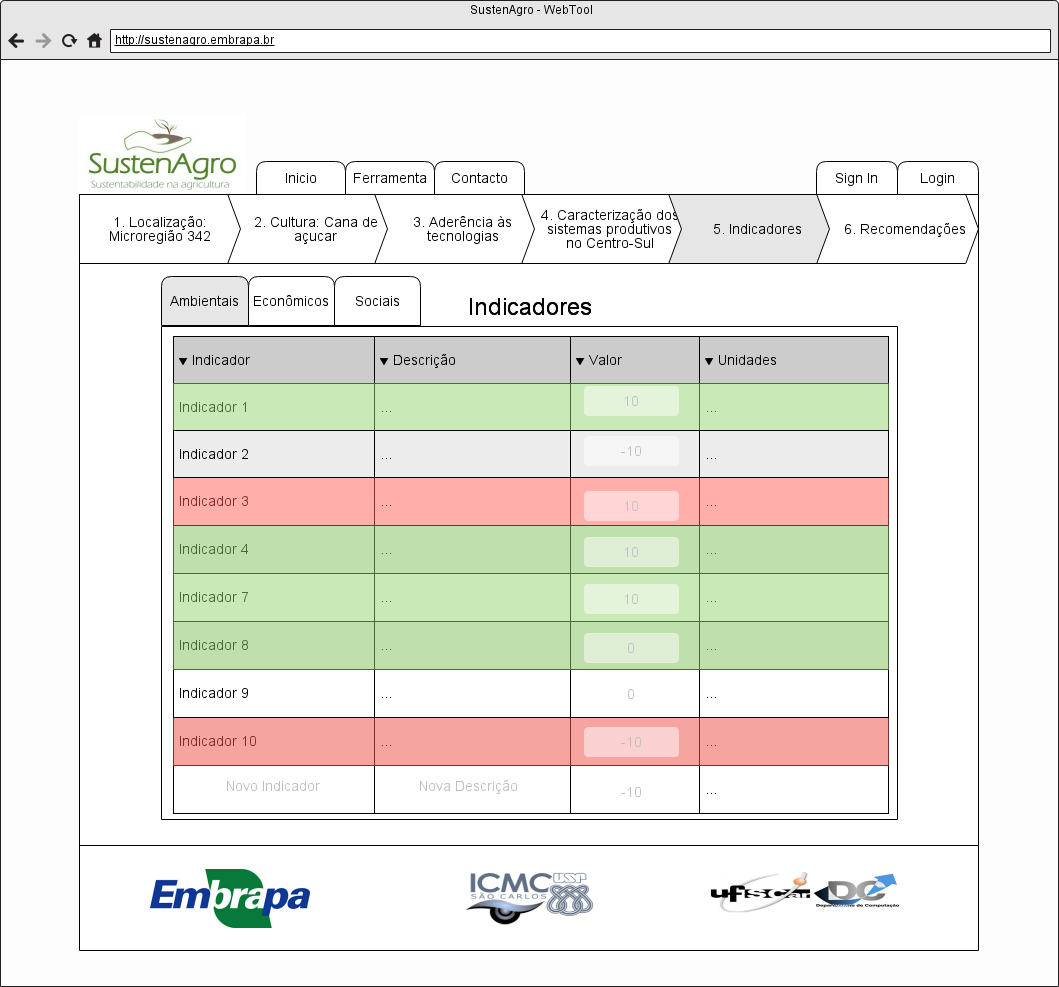
\includegraphics[width=1\columnwidth]{figures/Tool_environmental_indicators}\caption{Mockup da tela de indicadores do SustenAgro.\label{fig:Mockup_indicators}}
\end{figure}


\subsection*{Protótipo da Interface Gráfica do SustenAgro}

O protótipo funcional da interface gráfica do SustenAgro está disponível
nos servidores do laboratório Intermídia do ICMC\nobreakdash-USP
\footnote{http://biomac.icmc.usp.br:8080/sustenagro/}. Na Figura
\ref{fig:Home} é apresentada a página inicial do protótipo.

\begin{figure}[H]
\begin{centering}
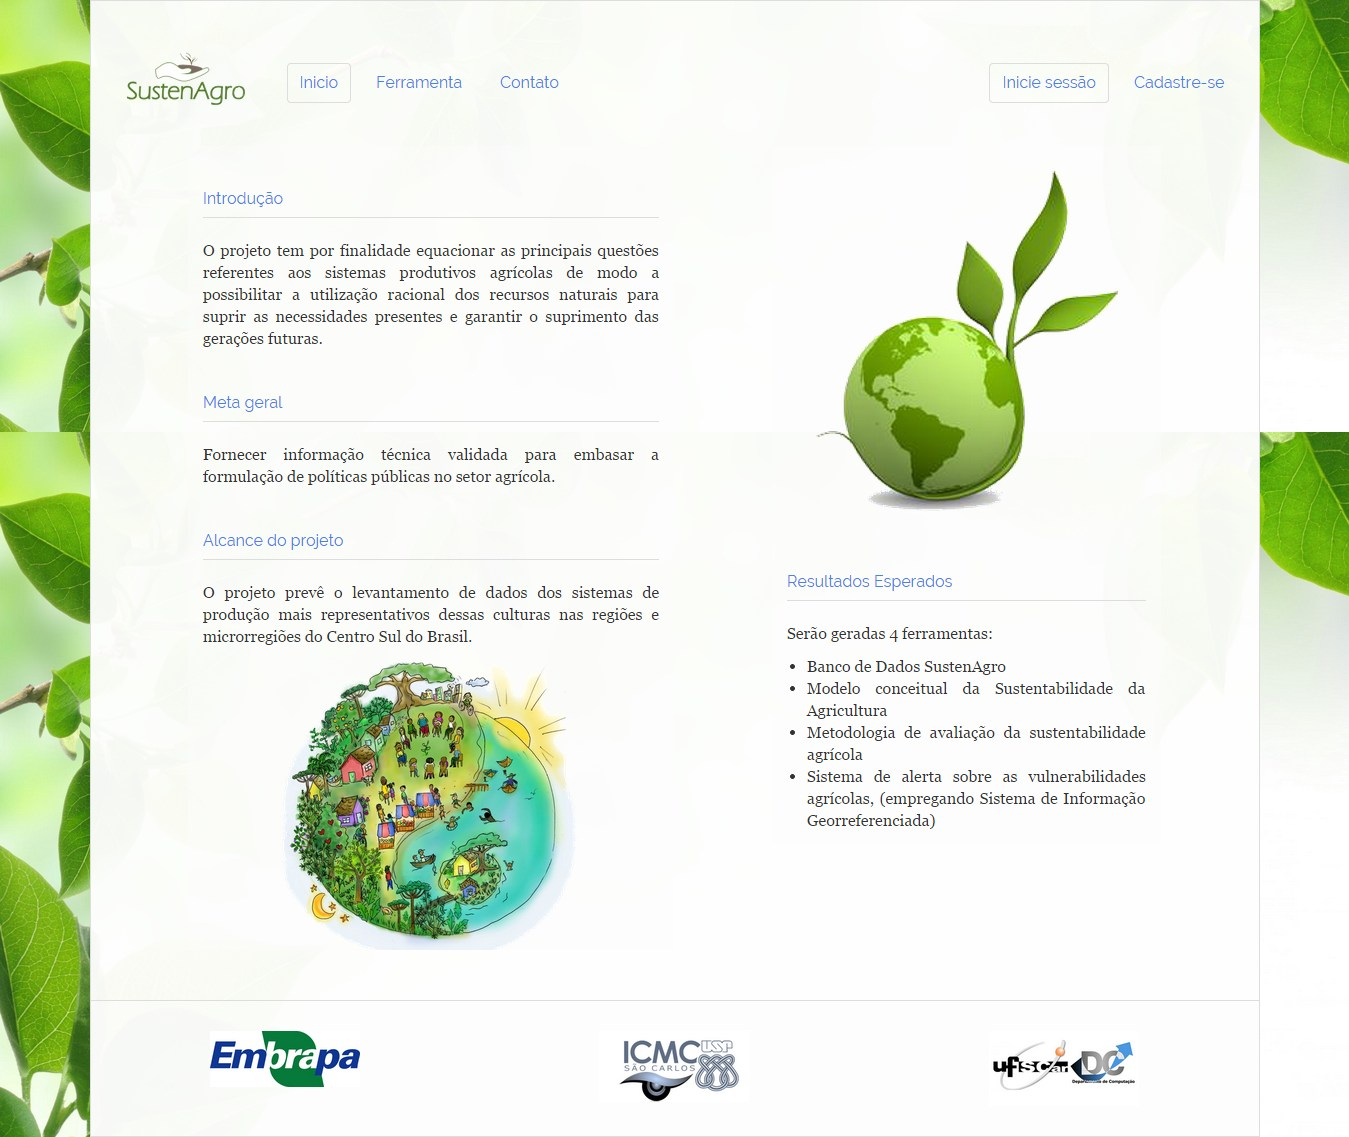
\includegraphics[width=1\textwidth]{figures/home}
\par\end{centering}
\caption{Protótipo do SustenAgro – Home Page.\label{fig:Home}}
\end{figure}

Nessa tela pode-se observar o texto explicativo da ferramenta e as
abas de ``Início'', ``Ferramenta'' e ``Contato''. A opção ``Ferramenta''
permite iniciar o processo de avaliação de sustentabilidade.

Uma vez cadastrada uma unidade produtiva, disponibiliza-se a opção
de criar nova avaliação. Essa, ação vai gerar a tela da Figura \ref{fig:Indicators},
que permite visualizar os indicadores para que os usuários preencham
cada um, segundo a realidade da unidade produtiva em avaliação. Cada
indicador tem várias opções de resposta que estão ligadas a valores
que quantificam a sustentabilidade. Esses valores estão definidos
na ontologia de sustentabilidade (a ontologia SustenAgro) e são usados
nas fórmulas para gerar os índices de sustentabilidade. 

Na Figura \ref{fig:Indicators}, é apresentado o formulário dos indicadores
de eficiência. Eles são subdivididos em eficiência de produção e tecnológica.
Na Figura \ref{fig:Indicators}, é mostrado o indicador Manejo, como
exemplo. Um tipo de manejo foi escolhido e o peso desse indicador
foi declarado como direto. Esses valores serão usados nas fórmulas
da avaliação da sustentabilidade.

\begin{figure}[H]
\noindent \begin{centering}
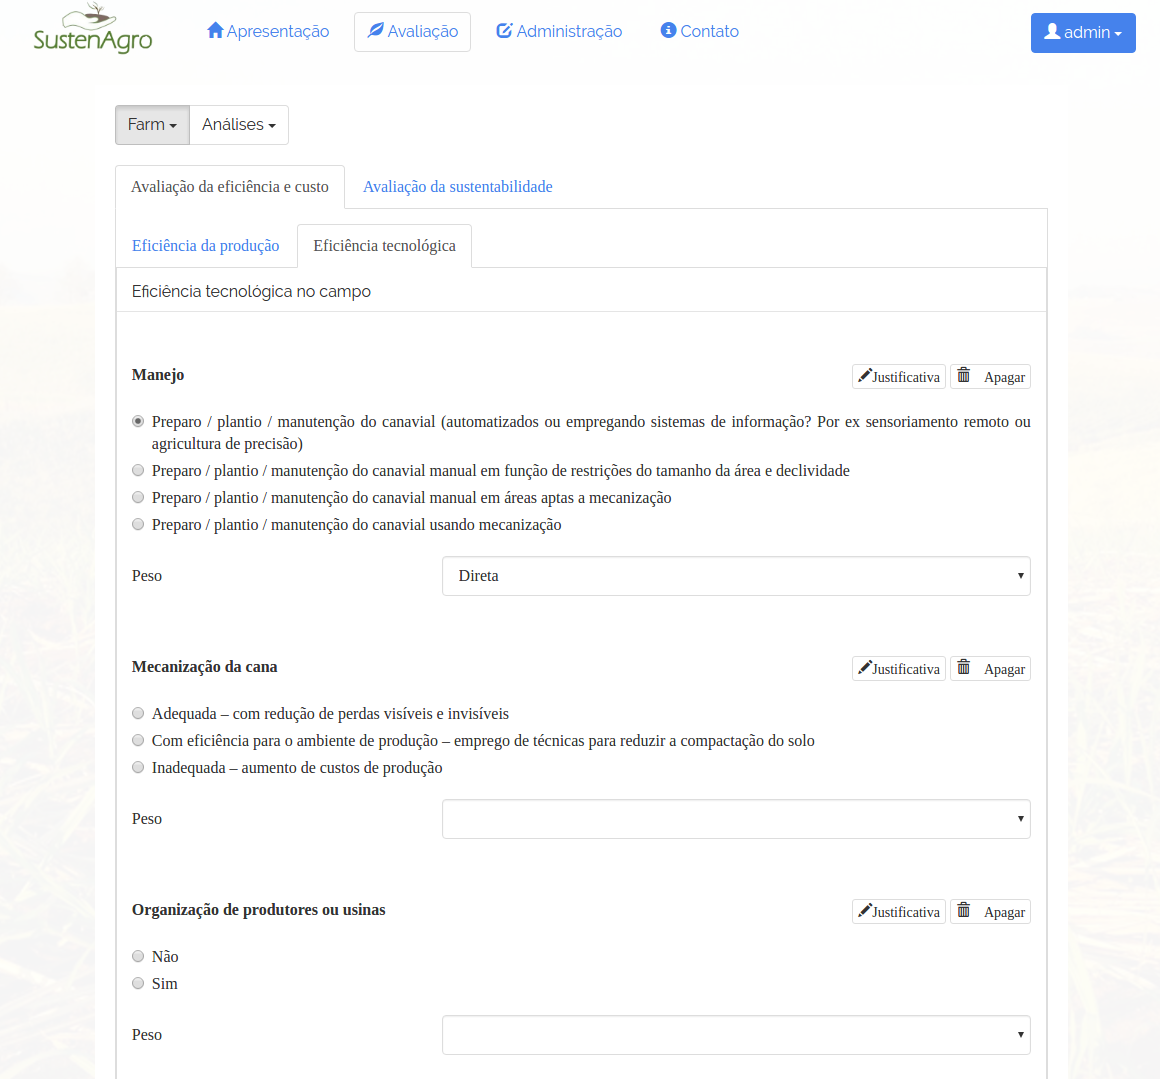
\includegraphics[width=1\columnwidth]{figures/SustenAgro-scenario}
\par\end{centering}
\caption{Cadastro de indicadores \label{fig:Indicators}}
\end{figure}

A partir dos dados cadastrados, são gerados os resultados do sistema.
Eles consistem na planilha de eficiência e custo, na planilha da sustentabilidade
e o relatório do sistema. As planilhas permitem visualizar os atributos
dos indicadores e a tela de relatório apresenta a matriz de sustentabilidade,
onde são relacionados os índices de eficiência e de sustentabilidade.
O relatório é apresentado na Figura \ref{fig:Planilhas-de-resultado}. 

\begin{figure}[H]
\noindent \begin{centering}
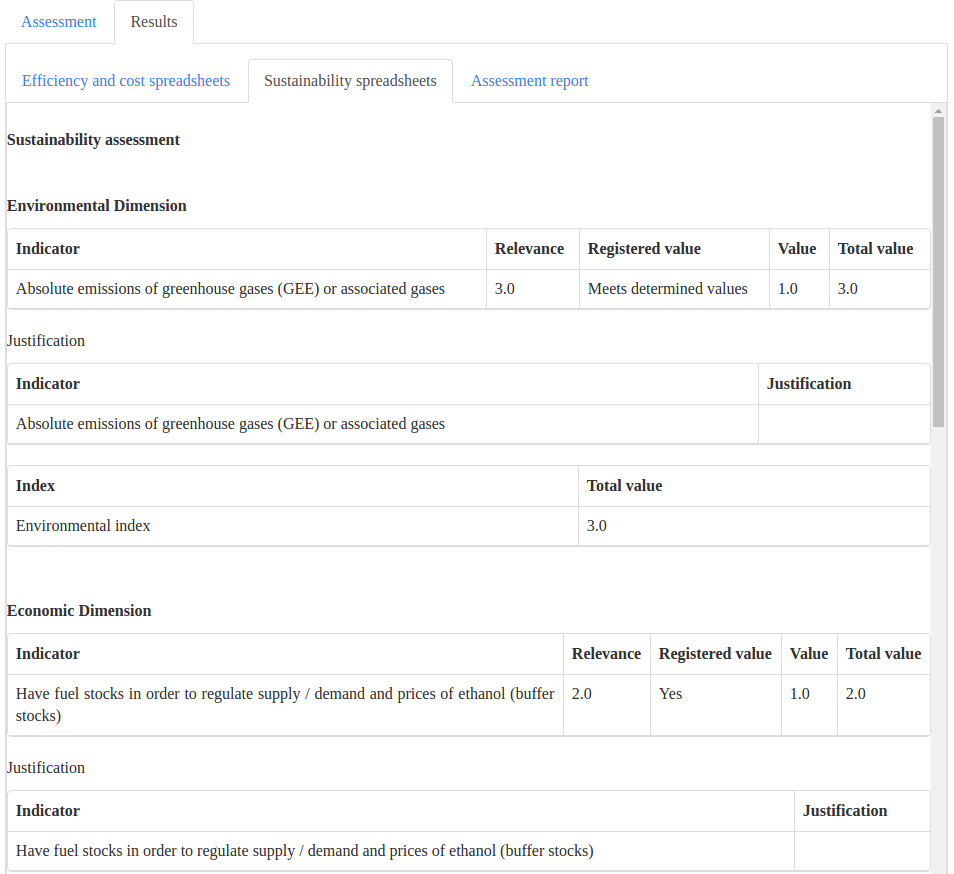
\includegraphics[width=1\columnwidth]{figures/SustenAgro-results}
\par\end{centering}
\caption{Planilhas do resultado da avaliação \label{fig:Planilhas-de-resultado}}
\end{figure}

\selectlanguage{english}%

\section{Web Components}

\selectlanguage{brazil}%
Foram desenvolvidos dois \foreignlanguage{english}{Web Components}
específicos para o SustenAgro. Eles geram gráficos específicos do
relatório solicitado pelos especialistas da Embrapa Meio Ambiente 

\subsection*{Matriz de Sustentabilidade}

Com a finalidade de suportar a geração de relatórios, no formato definido
pelos especialistas do domínio, foi necessário implementar dois \foreignlanguage{english}{Web
Component} especificos. Um deles foi a \foreignlanguage{english}{widget}
intitulada Matriz de Sustentabilidade. Ela é composta por dois eixos
que correspondem ao índice de eficiência, eixo Y, e ao índice de sustentabilidade,
eixo X. Os índices tem magnitudes que são dividas em segmentos que
permitem dividir a área em doze quadrantes da sustentabilidade. Cada
avaliação realizada com o método SustenAgro gerará dois índices que
são localizados em um quadrante da matriz de sustentabilidade. Cada
quadrante está relacionado com uma recomendação específica. A Figura
\ref{fig:Matriz-de-sustentabilidade} mostra a implementação desse
\foreignlanguage{english}{Web Component,} mostrando resultados reais
de uma avaliação.

\begin{figure}[H]
\noindent \begin{centering}
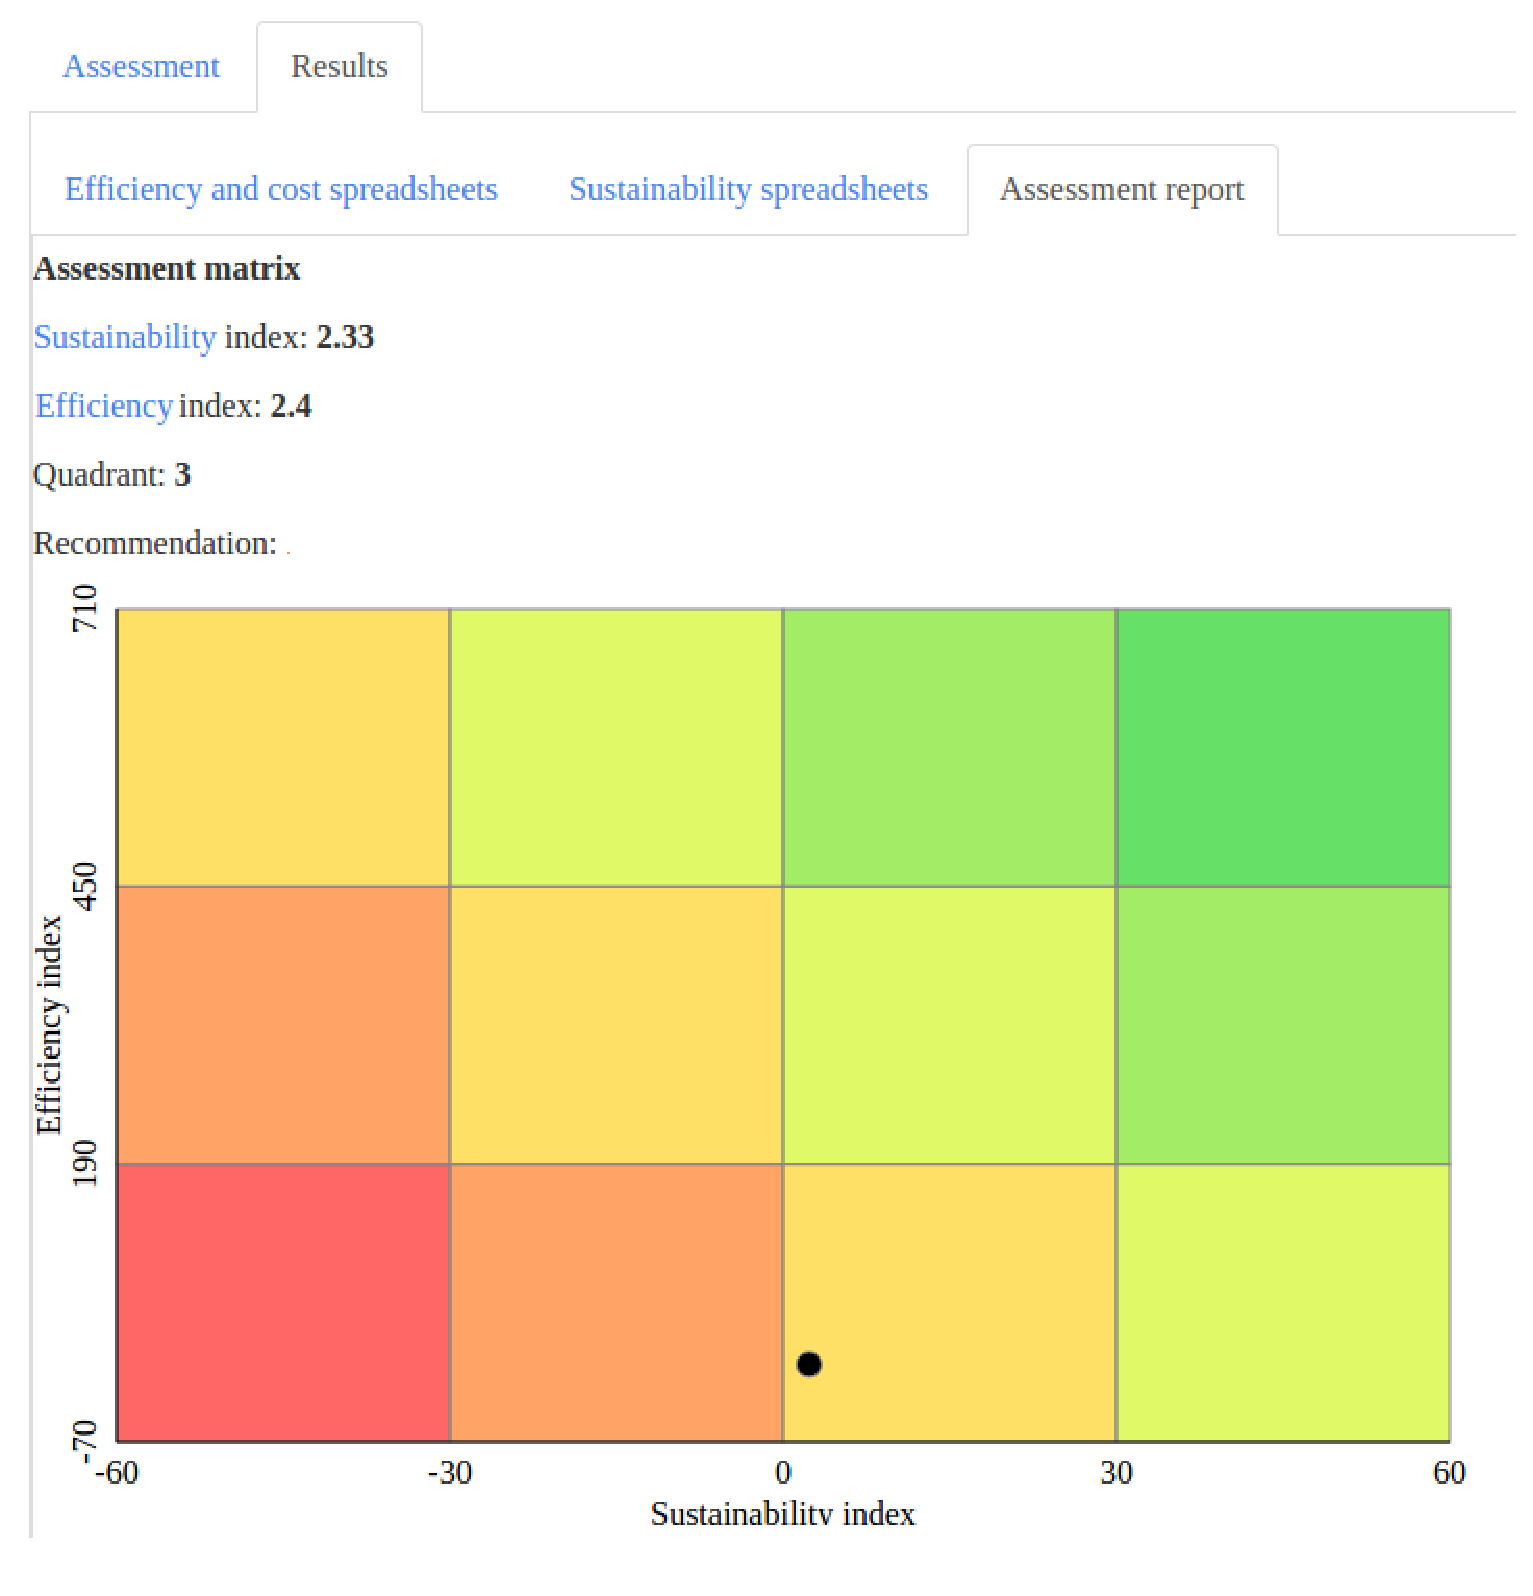
\includegraphics[width=1\columnwidth]{figures/SustenAgro-matrix}
\par\end{centering}
\caption{Matriz de sustentabilidade\label{fig:Matriz-de-sustentabilidade-widget}}
\end{figure}


\subsection*{Semáforo da Sustentabilidade}

O \foreignlanguage{english}{Web Component} do Semáforo da Sustentabilidade
foi o segundo componente para geração de relatórios, no formato definido
pelos especialistas do domínio, desenvolvido para o método SustenAgro.
Ele tem um eixo que quantifica o valor da sustentabilidade normalizado
entre -100 até +100, dividindo o intervalo em 5 segmentos que correspondem
às categorias de sustentabilidade. A Figura \ref{fig:Sem=0000E1foro-de-sustentabilidade}
mostra esse componente no sistema SustenAgro com os valores para uma
avaliação de sustentabilidade.

\begin{figure}[H]
\noindent \begin{centering}
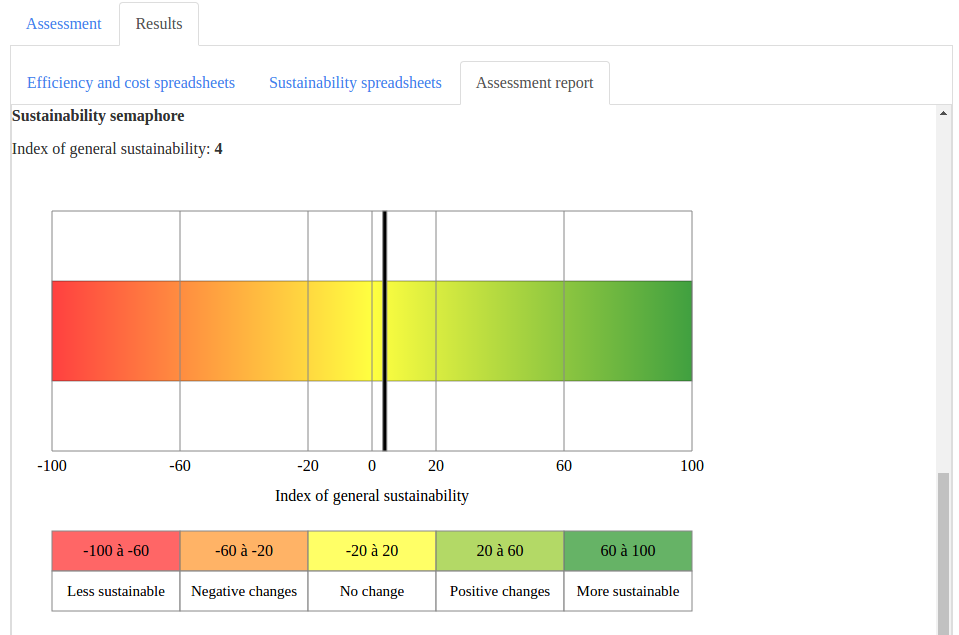
\includegraphics[width=1\columnwidth]{figures/SustenAgro-semaphore}
\par\end{centering}
\caption{Semáforo de sustentabilidade \label{fig:Sem=0000E1foro-de-sustentabilidade}}

\end{figure}

\selectlanguage{english}%

\section{DSL: code}

\selectlanguage{brazil}%
A implementação de uma DSL permite aos especialistas do domínio definir
como são usados e apresentados os conceitos da ontologia, por meio
de elementos da interface gráfica, como os índices de sustentabilidade
serão calculados e quais os elementos presentes no relatório final.
A DSL permite a criação de SADs facilmente adaptáveis às mudanças
do domínio. Os próprios especialistas podem modificá-la sem o auxílio
de programadores.

Para definir o comportamento do SustenAgro, especialistas tiveram
que:

\subsection{Definir o Objeto da Avaliação}

No comando, a seguir, o Objeto de Avaliação é definido como uma instância
da classe ProductionUnit. Essa classe foi definida pelos próprios
especialistas na ontologia e tem como filhos as classes . Também
são declaradas todas as propriedades que os usuários terão que preencher
quando criarem uma avaliação. Por exemplo, na propriedade \textit{hasName}
os usuários devem preencher o nome da unidade de produção.

\inputencoding{latin9}\begin{lstlisting}
evaluationObject ':ProductionUnit', {             
  instance 'ui:hasName', label: ['en': 'Production unit or farm name', 'pt': 'Nome da unidade produtiva ou fazenda'], placeholder: ['en': 'Name', 'pt': "Nome"]
  instance ':hasAgriculturalProductionSystem', label: ['en': 'Agricultural production system' , 'pt': "Sistema de produ��o agr�cola"], header: ['en': 'Options', 'pt': "Op��es"]     
  type label: ['en': "Production unit type", 'pt': "Tipo da unidade produtiva"], header: ['en': 'Options', 'pt': "Op��es"]
  instance  ':hasSugarcaneSource', label: ['en': 'Sugarcane source', 'pt': "Origem da cana"], header: ['en': 'Options', 'pt': "Op��es"], multipleSelection: true, required: true
  instance 'dbp:state', label: ['en': 'State', 'pt': 'Estado'], header: ['en': 'States', 'pt': 'Estados']
  instance 'ui:hasMicroregion', label: ['en': 'Production unit microregion', 'pt': "Microrregi�o da unidade produtiva"], header: ['en': "Options", 'pt': "Op��es"]
  instance ':hasAvailabilityOfEvaluationResults', label: ['en': "Availability of evaluation results", 'pt': "Disponibiliza��o dos resultados da avalia��o"], header: ['en': "Options", 'pt': "Op��es"]
}
\end{lstlisting}
\inputencoding{utf8}

\subsection{Definir as características a serem avaliadas}

Agora os especialistas têm que escolher quais características (Features)
dos Objetos de Avaliação serão usadas. No comando \textit{feature},
são indicadas as classes das \textit{Features} a serem usadas. Serão
mostradas todas as \textit{features} das classes indicadas e de suas
descendentes. Por exemplo, o comando \textit{feature ':ProductionEfficiencyFeature'}
vai mostrar todas as \textit{Features} relacionadas com eficiência
da produção. Na ontologia SustenAgro foram estabelecidas as famílias
de \foreignlanguage{english}{\textit{Features}}: EnvironmentalIndicator,
EconomicIndicator, SocialIndicator, ProductionEfficiencyFeature e
TechnologicalEfficiencyFeature.

O comando \textit{feature} também permite dizer se existirão novas
\textit{Features} criadas pelos usuários ('extraFeatures': true) e
a apresentação condicional de grupos de Features. No exemplo da Listagem
, são mostradas Features industriais apenas à usuários de usinas.

\inputencoding{latin9}\begin{lstlisting}
feature ':EnvironmentalIndicator', 'extraFeatures': true 
feature ':EconomicIndicator', 'extraFeatures': true 
feature ':SocialIndicator', 'extraFeatures': true 
feature ':ProductionEfficiencyFeature' 
feature ':TechnologicalEfficiencyFeature', {          
  conditional ":ProductionUnit", 'http://dbpedia.org/ontology/Provider', {
    include ':TechnologicalEfficiencyInTheField'          
  }
  conditional ":ProductionUnit", 'http://dbpedia.org/resource/PhysicalPlant', {
    include ':TechnologicalEfficiencyInTheField', ':TechnologicalEfficiencyInTheIndustrial'          
  }  
}
\end{lstlisting}
\inputencoding{utf8}

\subsection{Definir o modelamento e a forma de apresentação dos resultados}

Finalmente, no comando \textit{data}, os especialistas definem o nome
da variável que contém as respostas dos usuários e, no comando \textit{report},
fazem o cálculo do modelamento e definem o que vai ser apresentado.
Na listagem , é possível ver o cálculo dos índices de sustentabilidade
e eficiência através das formulas do modelo usado pelo SustenAgro.
É possível usar qualquer comando da linguagem Groovy ou biblioteca
externa. As variáveis guardam os valores de interesse que serão mostrados
no relatório de avaliação. No caso do SustenAgro, a variável \foreignlanguage{english}{\textit{sustainability}}
guarda o índice de sustentabilidade e a variável \textit{efficiency}
guarda o índice de eficiência do sistema.

No relatório aparecerão a Matriz de Sustentabilidade (SustainabilityMatrix),
o Semáforo de Sustentabilidade (SustainabilitySemaphore), o texto
\textquotedbl{}Mapa da Microregião\textquotedbl{} e o mapa da microregião
(onde a unidade produtiva se encontra). Cada uma dessas widget é instanciada
na DSL e os valores de interesse são passados para os Web Components
encarregados da apresentação. O framework Decisioner delega aos Web
Components a tarefa de apresentação.

Usuários podem pedir a geração de relatórios em pdf, uma ferramenta
de conversão de HTML para pdf é usada.

\inputencoding{latin9}\begin{lstlisting}[caption={SustenAgro DSL },label={lis:DSL-SustenAgro}]
data 'data'
report {       
  environment =   weightedSum(data.':EnvironmentalIndicator')

  economic    =   weightedSum(data.':EconomicIndicator')     
 
  social      =   weightedSum(data.':SocialIndicator')  

  sustainability = (environment + social + economic)/3

  cost_production_efficiency = sum(data.':ProductionEfficiencyFeature')

  technologicalEfficiencyInTheField = 0.8*weightedSum(data.':TechnologicalEfficiencyInTheField')

  technologicalEfficiencyInTheIndustrial = 0.2*weightedSum(data.':TechnologicalEfficiencyInTheIndustrial')

  efficiency = Math.abs(cost_production_efficiency) * (technologicalEfficiencyInTheField+technologicalEfficiencyInTheIndustrial)

  sustainabilityMatrix x: sustainability, y: efficiency,  
                       label_x: ['en': 'Sustainability Index', 'pt': '�ndice de Sustentabilidade'],                 
                       label_y: ['en': 'Efficiency index', 'pt': '�ndice de Efici�ncia'],
                       range_x: [-43,43],
                       range_y: [-160,800],
                       quadrants: [4,3]                       
   
  sustainabilitySemaphore value: sustainability,                  
                          label: ['en': 'Sustainability Level', 'pt': '�ndice da sustentabilidade geral'],
                          legend: [['en': 'Lower sustainability', 'pt': 'Menos sustent�vel'],
                                  ['en': 'Negative changes', 'pt': 'Altera��es negativas'],
                                  ['en': 'Irrelevant changes', 'pt': 'Sem altera��o'],
                                  ['en': 'Positive changes', 'pt': 'Altera��es positivas'],                                     
                                  ['en': 'Higher sustainability', 'pt': 'Mais sustent�vel']],
                          range: [-60,60]    

  text 'en': 'Microregion map', 'pt': '**Mapa da microregi�o**'    

  map data.'Microregion'   
}     
\end{lstlisting}
\inputencoding{utf8}

\section{Considerações Finais}

O desenvolvimento do sistema Sustenagro satisfez uma necessidade presente
na unidade da Embrapa Meio Ambiente: um sistema de avaliação de sustentabilidade
em cana-de-açúcar no centro-sul do Brasil. O SAD SustenAgro representa
e permite complementar informações e dados do estado atual de sustentabilidade
nas fazendas e usinas. Ele produz relatórios com a finalidade de embasar
e formalizar políticas para promover práticas produtivas mais sustentáveis,
de acordo com critérios ambientais, sociais e econômicos.

Além de satisfazer uma necessidade institucional, o SustenAgro é uma
proposta de SAD baseado em conhecimento e vinculado às tecnologias
da web semântica. O SustenAgro não foi apenas uma instanciação do
framework Decisioner, ele definiu o próprio framework. Através do
desenvolvimento do SustenAgro, foi possível determinar as características
gerais desse tipo de SAD, e implementá-las no framework, e as características
específicas do Sustenagro, que foram implementadas usando a ontologia
SustenAgro, os dois Web Components e a DSL.

Tendo o sistema SustenAgro instanciado e rodando, foi possível validar
suas funcionalidades através de alguns experimentos com integrantes
do projeto SustenAgro da Embrapa. Os resultados obtidos nas avaliações
dos experimentos serão detalhados no próximo capítulo.
